\documentclass{book}
\usepackage{amsmath, amsthm, graphicx, amsfonts, float}
\usepackage[english]{babel}
\graphicspath{ {./images/} }

\usepackage{geometry}
 \geometry{
 a4paper,
 total={170mm,237mm},
 left=20mm,
 top=30mm,
 }
 \usepackage[hidelinks]{hyperref}

\newcommand\at[2]{\left.#1\right|_{#2}}
\DeclareMathOperator{\sgn}{sgn}
\newcommand{\notimplies}{%
  \mathrel{{\ooalign{\hidewidth$\not\phantom{=}$\hidewidth\cr$\implies$}}}}


\title{Industrial Robotics M}
\author{Dante Piotto}
\date{spring semester 2023}


\begin{document}

\maketitle
\tableofcontents

\chapter{Elements of Kinematics and Dynamics of Industrial Robots}

\section{Introduction}
A manipulator may be mechanically described as the interconnection of rigid bodies \emph{(links)} through kinematic pairs \emph{(joints)}. In this course we deal with open chains of links (serial configuration). The first link is the \emph{base}, while the last link is the \emph{end effector}. We will consider the links to be rigid bodies for the sake of simplicity.

A joint is an element that constrains one or more relative motion directions between two links.
In robotics only two types of joints are used: rotoidal joints and prismatic joints.
\subsection{Degrees of Freedom of a Manipulator}
Each joint is characterised by the number of independent motion directions allowe between two consecutive links. This number defines the \emph{degrees of freedom} of the joint. Rotoidal and prismatic joints have 1 degree of freedom (dof of the joint. Rotoidal and prismatic joints have 1 degree of freedom (dof).
In place of spehrical joints, 3 rotoidal joints are used, forming a \emph{spherical wrist}. The spherical wrist is typically at the end of the kinematic chain.
%insert image of spherical wrist
If a joint has $k$ dof, then the relative configuration between two rigid bodies may be expressed as a function of $k$ variables $q_1, q_2, \dots, q_k$, called \emph{joint variables}.




\subsection{Joint Space and Work Space}
Joint Space: Let us stack all the joint variables in a vector \[q= \begin{bmatrix}
    q_1 & q_2 & \dots & q_n
\end{bmatrix}^T\] with $q\in \mathcal{Q}\subset \mathbb{R}^{N_dof}$. The set $\mathcal{Q}$ is called \emph{joint space}

Work Space: The work space is a subset of the Euclidean space $\mathbb{E}$ in which the robot executes its tasks. It is the set of all the points that the mechanical structure may assume, and in general is a 3D subset of $\mathbb{E}$. Each point of the work space is indicated by a vector $x$ of proper dimension, $x\in \mathbb{R}^y$, where usually $y=\{3,6\}$

configuration of a manipulator: It takes into account both the position and orientation of a reference frame  fixed to the manipulator extremity (end effector). Then (locally): \begin{itemize}
    \item $x\in\mathbb{R}^3$ in a plane
    \item $x\in\mathbb{R}^6$ in space
\end{itemize}

Classification of manipulators: if $\mathbb{R}^n$ is the joint space and $\mathbb{R}^m$ is the work space:
\begin{itemize}
    \item $n=m$: "normal" cases
    \item $n<m$: \emph{defective} manipulators
    \item $n>m$: \emph{redundant} manipualtors
\end{itemize}



\subsection{Types of Robotic Manipulators}

Common kinematic structures for robotic manipulators:
\begin{itemize}
    \item Cartesian robots: 3 perpendicular prismatic joints. Simplest robot structure. Structure can be made to be very robust and therefore very large. Usually meant to move large payloads. Simple to control (1 motor for each direction of motion). Simple mapping between joint space and work space.
    \item Antropomorphic robots (majority): 3 rotational joints, 1 with a vertical axis and 2 with horizontal axes. More dexterous, harder to control, more complex coupling between joint space and work space. Errors on eaech motor stack in the final motion
    \item SCARA robots: Selective Compliance Assembly Robot Arm. Rigid along z, more compliant along x and y.
    \item Cylindrical and spherical robots: not used
    \item Spherical wrists: typically attached at the end of Cartesian, Antropomorphic or SCARA bots.
\end{itemize}
The first 3 joints define the basic kinematic structure
%insert images



\section{Kinematic model of a manipulator}

x is made of 3 elements determining position an 3 determining orientation. These 3 represent angles, taht may be Roll-Pitch-yaw, or Euler angles (Z-Y-Z Euler angles are used in robotics) 

\subsection{Forward kinematics}
mapping of joint space variables into work space variables
\[
    x=f(q) \quad q\in \mathbb{R}^n, x\in \mathbb{R}^m
\]
It is possible to define different kinematic models for a robotic manipulator, i.e. different $f(q)$ functions. They are however mathematically equivalent
\subsubsection{Homogenous trasformation matrix}
the configuration of a rigid body $b_i$ in a 3D space can be described by a \emph{homogenous transformation matrix} betweeen a reference frame $FF_i$ and the base frame $FF_0$ thus constructed: 
\[
    ^0T_i=\begin{pmatrix}
        ^0R_i & ^0o_i\\
        \mathbf{0} & 1
    \end{pmatrix}
\]

where $^0R_i$ is a rotation matrix belonging to $SO(3)$, and $^0o_i\in\mathbb{R}^3$ is a position vector. It can be noted that the determinant of the homogenous transformation matrix is also equal to 1.

For computational reasons, a new position vector $p=[p_x,p_y,p_z,1]^T$ is defined. This way, the position $^0p$ of a generic point $^1p$ of the rigid body can be obtained as:
\[
    ^0p=^0T_1 {^1}p
\]
or, with some abuse of notation:
\[
    \begin{bmatrix}
        ^0p \\ 1
    \end{bmatrix} = ^0T_1 \begin{bmatrix}
        ^1p \\ 1
    \end{bmatrix} = \begin{bmatrix}
        ^0R_1 {^1}p + ^0o_1\\
        1
    \end{bmatrix}
\]

in general
\[
    ^0T_n = ^0T_1 {^1}T_2 \dots ^{n-1}T_n
\]
due to homogenous transformation being a linear operation.

\subsubsection{Denavit-Hartenberg convention}
\begin{itemize}
    \item each link is numbered, from $0$ to $n$, so that it is uniquely identified in the mechanical chain: $L_0, L_1, \dots, L_n$. The base link is conventionally identified as $L_0$, the distal link as $L_n$. A manipulator with $n+1$ links has $n$ joints.
    \item Joints are numbered from $1$ to $n$. $J_i$ connects links $L_{i-1}$ and $L_i$
    \item Frames $\mathcal{F}_i$ are associated to each joint, according to the Denavit-Hartenberg procedure, and matrices $^{i-1}T_i$ are computed:\begin{itemize}
        \item all the z axes are directed along the direction of motion
        \item axis $x+1$ intersects and is perpendicular to axis $z_i$
    \end{itemize}
    \item The Denavit-Hartenberg procedure requires 4 parameters for each link ($d_i, \theta_i, a_i, \alpha_i$)
\end{itemize}

This procedure provides a 4x4 matrix, not a vector, for $x$. The vector $x$ can be computed as a function of the homogeneous trasformation matrix.





\subsection{Inverse kinematics}
mapping of work space variables into joint space variables
\[
    q=g(x)=f^{-1}(x) \quad q\in \mathbb{R}^n, x\in \mathbb{R}^m
\]
A standard procedure to obtain the inverse kinematic model does not exist.\\
Moreover, we may have 
\begin{itemize}
    \item no solution (if x does not belong to the workspace
    \item a finite set of solutions
    \item infinite solutions
\end{itemize}
A \emph{closed form} solution is preferrable to numerical procedures (better computation, easier to select a particular solution in the set of solutions)\\
A closed form solution to the inverse kinematic problem may be obtained, if it exists, by trying one of these approaches:
\begin{itemize}
    \item Algebraic approach: elaboration of the kinematic equatoins in order to obtain a set of 'simple' equations that can be solved in the uknown joint variables $q$
    \item Geometric approach: based on considerations dependent on the geometric structure of the manipulator
\end{itemize}
\subsubsection{Algebraic approach}
The values of the homogenoeus trasnformation matrix are known, and the homogeneous trasnformation matrix can be written as a function of joint variables. This yields 12 scalar equations (usually more than needed). Hopefully there are a sufficient number of equations that can be solved easily enough. As an additional resource, one can perform algebraic manipulations on the involved matrices to try and find a better set of equations. 
This procedure is in general not so simple

\subsubsection{Geometric approach}
Also called Pieper approach.\\
For several kinematic structures it is possible to apply the \emph{kinematic decoupling} principle, that allows to decompose the overall 6Dof problem into two 3 Dof sub-problems:
\begin{itemize}
    \item inverse kinematic problem for position
    \item inverse kinematic problem for orientation 
\end{itemize}
Sufficient condition to solve the inverse kinematic problem for a 6DoF manipulator:
\begin{itemize}
    \item 3 consecutive rotational joints whose axes intersect in a point (spherical wrist: notice that the position of the center of rotation of the spherical wrist does not depend on the joint variables of the spherical wrist but rather on the other joints)
    \item 3 consecutive rotation joints with parallel axes
\end{itemize}





\subsection{Differential kinematics - the Jacobian}
Ohter relations of intrest in robotics are those between:
\begin{itemize}
    \item end-effector velocity and joint velocities $$\begin{pmatrix} v \\ \omega \end{pmatrix} \iff \dot{q}$$
    \item force applied on the environment by the manipulator and corresponding joint torques:
    $$ \begin{pmatrix} f \\ n \end{pmatrix} \iff \tau $$
\end{itemize}
These relations are based on a matrix known as the \emph{Jacobian of the manipulator}. The Jacobian is also used for:
\begin{itemize}
    \item studying the singularities of the mechanical structures
    \item defining numerical algorithms to solve the inverse kinematics
    \item studying manipulability properties
\end{itemize}

The six-dimensional velocity vector (twist) in the woek-space is defined with three linear and three rotational components
\[
    \dot{x}=\begin{pmatrix} v \\ \omega \end{pmatrix}
\]
Two expressions of the Jacobian matrix can be defined:
\begin{itemize}
    \item the analytic Jacobian, used when the rotational component in $\dot{x}$ is defined as $\dot{\gamma}$, the time-derivative of a triple of orientation variables
    \item the geometric Jacobian, used when the rotational component in $\dot{x}$ is defined as $\omega$, the rotational velocity vector.
\end{itemize}
It is possible to relate the two expressions by means of a proper matrix $T(\gamma)$
\[
    J_G(q)=T({\gamma})J_A(q)=\begin{bmatrix}
        I_3 & 0 \\
        0 & \hat{T}(\gamma)
    \end{bmatrix}
    J_A(q)
\]
\subsubsection{Analytic Jacobian}
The analytic expression of the Jacobian is obtained by differentiating the six-dimensional vector $x=f(q)=[p^T,\gamma^T]^T$ containing the position ($p$) and orientation ($\gamma$) of the end-effector in the work-space wrtnthe base frame FF0; usually $\gamma$ are the Euler or RPY angles\\
By differentiating $f(q)$ we get:
\[
    dx=\frac{\partial f(q)}{\partial q}dq=J(q)dq \qquad (\dot{x}=J(q)\dot{q})
\]
where the $m\times n$ matrix
\[
    J(q)=\begin{pmatrix}
        \frac{\partial f_1}{\partial q_1} & \frac{\partial f_1}{\partial q_2} & \dots & \frac{\partial f_1}{\partial q_n}\\
        \vdots & \vdots &\ddots & \vdots \\
        \frac{\partial f_m}{\partial q_1} & \frac{\partial f_m}{\partial q_2} & \dots & \frac{\partial f_m}{\partial q_n}
    \end{pmatrix}, \qquad J(q) \in \mathbb{R}^{m\times n}
\]
Is called the \emph{Jacobian matrix}\\
We have that the relationship between $\dot{x}$ and $\dot{q}$ is linear.
The Jacobian can be conceptually split in two blocks, the first concerning the linear part of the velocity, the second concerning the angular part:
\[
    \dot{x}_A=J_A(q)\dot{q} = \begin{bmatrix} \dot{p} \\ \dot{\gamma} \end{bmatrix} = \begin{bmatrix} J_p \\ J_{\gamma} \end{bmatrix} \dot{q}
\]

\subsubsection{Geometric expression}
In practice, the Jacobian is always computed in its geometric expression as it is much simpler. The geometric expression of the Jacobian is obtained considering as rotational components of the velocity vector $\dot{x}$ the rotational vector $\omega$ and not the derivative of a triple of angles $\gamma$
\[
    \dot{x}=\begin{bmatrix} \dot{p} \\ \dot {\gamma} \end{bmatrix} \quad \iff \quad \dot{x}=\begin{bmatrix} \dot{p} \\ \omega \end{bmatrix}
\]

\[
    \dot{x}_G=J_G(1)\dot{q}=\dot{x}=\begin{bmatrix} \dot{p} \\ \omega \end{bmatrix} = \begin{bmatrix} J_v \\ J_w \end{bmatrix} \dot{q}=\begin{bmatrix}
    J_{v_1} & J_{v_2} & \dots J_{v_n}\\ 
    J_{\omega_1} & J_{\omega_2} & \dots J_{\omega_n} 
\end{bmatrix}
\]
this leads to 
\begin{gather*}
    v= J_{v_1}\dot{q}_1 + J_{v_2}\dot{q}_2 + \dots + J_{v_n} \dot{q}_n \\
    \omega= J_{\omega_1}\dot{q}_1 + J_{\omega_2}\dot{q}_2 + \dots + J_{\omega_n} \dot{q}_n \\
\end{gather*}
it is possible to show, applying the superimposition principle by considering only the $i-th$ joint to be moving, that the generic $i-th$ column of the geometric Jacobian is defined as
\[
    \begin{bmatrix} J_{vi} \\ J_{\omega i} \end{bmatrix} = \begin{bmatrix}
    ^0z_{i-1} \times (^0p_n-^0p_{i-1}) \\
    ^0z_{i-1}
\end{bmatrix} \qquad \text{rotational joint}
\]
\[
    \begin{bmatrix} J_{vi} \\ J_{\omega i} \end{bmatrix} = \begin{bmatrix}
    ^0z_{i-1}\\
    0
\end{bmatrix} \qquad \text{rotational joint}
\]
Once the forward kinematics of the manipulater is know these expressions are simple to obtain as the vectors $^0p_i$ and $^0z_i$ are obtained from the matrices $^0T_i$. This does not represent a computational burden with respect to the computation of the forward kinematic model.
\subsubsection{Force domain}
By exploiting the \emph{virtual work principle}, a mapping similar to that in the velocity domain can be obtained for the force domain.\\
Because work is invariant wrt the frame in which it is computed:
\[
    w^Tdx=\tau^Tdq
\]
where $w=(f^T n^T)^T$ is a 6-dimensional vector (\emph{wrench}) collecting the linear forces $f$ and the torques $n$ applied to the manipulator. $\tau$ is the n-dimensional vector of the \emph{joint forces/torques}
since 
\[
    dx=J(q)dq
\]
we obtain by substituting
\[
    \tau = J^T(q)w
\]
\subsubsection{Singularities}
When the Jacobian is rank deficient, there are directions in $\mathbb{R}^6$ that the robot cannot move in. Furthermore, limited velocities of the end-effector may correspond to infinite veolocities in the joint space. There is no well defined solution to the inverse kinematic problem: either no solution or infinite solutions. Singularities typically correspond to positions at the border of the workspace.\\
\subsubsection{Inverse differential kinematics}
The forward mapping betweeen joint and work-space is given by 
\[
    \dot{x}=J(q)\dot{q}
\]
Then, the inverse mapping is given as the solution of a linear algebraic equation
\begin{itemize}
    \item $m=n$: if the manipulator is not in a singular configuration, it is possible to use the inverse of the jacobian: \[
            \dot{q}=J^{-1}(q)\dot{x}
        \]
    \item $m \neq n$: the Moore-Penrose pseudoinverse of the Jacobian is used:
        \[
            \dot{q}=J^\dagger(q)\dot{x}
        \]
\end{itemize}
if $m<n$ (right pseudoinverse):
\begin{gather*}
    J^\dagger = J^T(JJ^T)^{-1}\\
    J^\dagger=I_m
\end{gather*}
if $m>n$ (left pseudoinverse):
\begin{gather*}
    J^\dagger=(J^T J)^{-1}J^T\\
    J^\dagger=I_n
\end{gather*}
When the joint space is larger than the work space ($n>m$), the solution of $\dot{x}=J\dot{q}$:
\begin{itemize}
    \item $rank(J)=min(m,n)=m \quad \implies \mathcal{R}(J)=\mathbb{R}^m$
    \item $\forall \dot{x}, \exists \dot{q} \text{ such that } \dot{x}=J\dot{q} \quad \text{ more than one exists}$
    \item $\dot{q}=J^\dagger \dot{x}+\dot{q}_N \implies \dot{x}=J(J^\dagger \dot{x} + \dot{q}_n=\dot{x} \quad \forall \dot{q}_N in \mathcal{N}(J)$ \\
        $\implies \dot{q} = J^\dagger \dot{x} + (I-J^\dagger J)y$ is a general expression of the solution
        \\$(I-J^\dagger J)$ is a base of $\mathcal{N}(J)$
    \item $\dot{q}=J^\dagger \dot{x}$ has \emph{minimum norm}
\end{itemize}

\subsubsection{Inverse kinematics with the Jacobian}
The Jacobian may be used to solve the inverse kinematic problem if a closed form solution is not available. A method could be to compute
\[
    q_{k+1}=q_k+J^{-1}(q_k)v_k dt
\]
where a numerical integration of the position is performed. Unfortunately, this method is subject to numerical drifts and initialization problems, and it is therefore difficult to obtain the desired solution. 

An alternative method is based on a feedback loop, by defining an error in the work-space. Given
\[
    e=x_d-x
\]
by differentiating, we obtain
\[
    dot{e}=\dot{x}_d-J(q)\dot{q}
\]
it is necessary to define $\dot{q}$ in such a way that the error $e$ converges to $0$
\subsubsection{Algorithm 1}
if
\[
    \dot{q}=J^{-1}(q)(\dot{x}_d+Ke)
\]
with $K=K^T>0$, then
\begin{gather*}
    \dot{e}=\dot{x}_d-JJ^{-1}(\dot{x}_d+Ke)\\
    \dot{e}=-Ke
\end{gather*}
Typically $K$ is chosen as a diagonal matrix, leading to
\begin{gather*}
    \begin{bmatrix}
        \dot{e}_1 \\
        \dot{e}_2 \\
        \vdots \\
        \dot{e}_n
        \end{bmatrix}=\begin{bmatrix}
        K_1 & \dots & & \\
        \vdots & K_2 & & \\
               & & \ddots & \\
        & & & K_n
    \end{bmatrix} 
    \begin{bmatrix}
        e_1 \\
        e_2 \\
        \vdots \\
        e_n
        \end{bmatrix} \\
    \end{gather*}
Which is completely decoupled and converging to 0.
%insert picture of control scheme
\subsubsection{Algorithm 2}
We use a Lyapunov technique:\\
Given $\dot{x}_d=0$, if
\[
    \dot{q}=J^T(q)Ke
\]
with $K=K^T>0$, then
\begin{gather*}
    V(e)=\frac{1}{2}e^TKe \implies \dot{V}(e)=e^TK\dot{e}=e^TK(\dot{x}_d-J\dot{q})\\
    =-e^TKJ(q)\dot{q}
\end{gather*}
we choose $\dot{q}=J^TKe$, leading to:
\[
    \dot{V}(e)=-e^TKJJ^TKe \leq 0
\]
%insert picture of control scheme



\subsection{Manipulability Measures}
The Jacobian may be used to evaluate the achievable performaces of a manipulator, in terms of velocities and applicable forces, through the \emph{manipulability ellipsoids}
\subsubsection{Velocity manipulability ellipsoids}
Given a sphere with unit radius radius in the joint velocity space, $\dot{q}^T\dot{q}=1$, that may be considered as a"cost" (energy input to the manipulator), we want to obtain its equivalent expression in the work-space. From $\dot{x}=J(q)\dot{q}$ we obtain:
\begin{gather*}
    \dot{q}=J^\dagger \dot{x}\\
    \implies \dot{x} J^{\dagger T}J^\dagger\dot{x}=1\\
    \implies \dot{x}^T(JJ^T)^\dagger\dot{x}=1
\end{gather*}
which is an ellipsoid in the work-space $\mathbb{R}^m$
\begin{itemize}
    \item the principal axes are directed along the eigenvectors of $JJ^T$
    \item the length of the principal axes are given by the singular values of J, $\sigma_i=\sqrt{\lambda_i(JJ^T)}$
\end{itemize}
\subsubsection{Force manipulability ellipsoids}
Let us now consider the equation $\tau^T\tau=1$ from which we obtain:
\[
    w^TJJ^Tw=1
\]
This equation describes an ellipsoid in the $\mathbb{R}^m$ force space
\begin{itemize}
    \item the principal axes are directed along the eigenvectors of $JJ^T$
    \item the length of the principal axes are given by the inverse of the singular values of J, $\sigma_i=\sqrt{\lambda_i(JJ^T)}$
\end{itemize}
This result confirms the duality of the velocity/force spaces: along the directions in which high velocity performances are possible, low force performances are achievable and viceversa

\chapter{Dynamic Model of Robotic Manipulators}
Dymanics of a robot manipulator: analysis of the relationship between the applied forces/torques and the resulting motion of a robot. For the dynamics, it is possible to define two "models":
\begin{itemize}
    \item Direct model: goven the forces/torques applied at joints, the hoint position and velocity, compute the acceleration
        \[
            \ddot{q}=f(q,\dot{q},\tau)
        \]
        and then
        \[
            \dot{q}=int \ddot{q} dy \qquad q= \int qdot{q}dt
        \]
    \item Inverse model: given the desired joint acceleration, velocity and position, compute the corresponding force/torque to be applied
        \[
            \tau = f^{-1}(\ddot{q},\dot{q},q)=g(\ddot{q},\dot{q},q)
        \]
\end{itemize}
In deriving the dynamic model of a robot, we refer to a chain of rigid bodies mutually, and ideally, connected among them
The dynamic model of a robot is used for:
\begin{itemize}
    \item simulation: testing motion behaviour without resorting to physical experiments
    \item analysis and synthesis of control laws
    \item alaysis of the structural properties of a manipulator in the design phase
\end{itemize}



\section{Euler-Lagrange model}
The dynamic model obtained through this method is simpler and more intuitive, and also better suited to understanding the effects of changes in the mechanical parameters. The links are considered altogether, and the model is obtained analytically. Drawbacks: the model is obtained starting from the kinetic and potential energies (non intuitive) and the model is not computationally efficient.

Lagrange coordinates: independet variables used to describe the position of rigid bodies in space. For the same physical system, several choices of Lagrangian coordinates are usually possible. In robotics, we use \emph{joint variables} $q_1,q_2,\dots,q_n$. Input torques should be defined according to the chosen Lagrangian coordinates $\implies$ joint torques $\tau_1,\tau_2,\dots,\tau_n$ 

From physics, we know it is possible to define:
\begin{itemize}
    \item the Kinetic Energy function $K(q\dot{q})$
    \item the Potential Energy function $P(q)$
\end{itemize}
And therefore the Lagrangian function 
\[
    \mathcal{L}(q\dot{q})=K(q,\dot{q})-P(q)
\]
The EEuler-Lagrange equations for a system described by $n$ Lagrange coordinates $q_i$ are
\[
    \psi_i=\frac{d}{dt}\left(\frac{\partial \mathcal{L}}{\partial \dot{q}_i}\right) - \frac{\partial \mathcal{L}}{\partial q_i} \qquad i=1,\dots,n
\]
Being $\psi_i$ the non-conservative (external or dissipative) generalized forces performing work on $q_i$. In robotics, we consider:
\begin{itemize}
    \item $\tau_i$ joint actuator torque
    \item $[J^TF_c]_i$ term due to external (contact) forces
    \item $d_{ii}$ $\dot{q}_i$ joint friction torque
\end{itemize}
Therefore:
\[
    \psi_i=\tau_i+[J^TF_c]_i-d_{ii}\dot{q}_i
\]

It can be noted that
\[
    K=\sum_{i=1}^{n}K_i \qquad P=\sum_{i=1}{n}P_i
\]

\subsection{obtained model}
\[
    M(q)\ddot{q} + C(q,\dot{q})\dot{q}+D\dot{q}+g(q)=\tau
\]
Non-linear wrt the state. It can be made linear wrt a set of parameters $\mathbf{\alpha}$

\subsection{Identification of the dynamic parameters}
From:
\[
    Y(q,\dot{q},\ddot{q})\alpha = \tau
\]
by measuring along a proper trajectory the quantities $q,\dot{q},\ddot{q}, \tau$ ($N>p$ samples) one obtains:
\begin{gather*}
    \tau_0=Y_0\alpha\\
    Y_0^T\tau_0 = Y_0^TY_0\alpha\\
    \alpha = (Y_0^TY_0)^{-1}Y_0^T\tau_0=Y_0^\dag \tau_0
\end{gather*}
\subsection{Dynamic model in simulink}
When only one of the two of the joints has friction energy still leaks out of the system because the system is coupled so movement of each link affects the other link causing the energy to be lost.
\subsection{Linearization of the Euler-Lagrange model}
By neglecting friction effects ($D=0$), and considering the vector $C(q,\dot{q})\dot{q} = c(q,\dot{q})$, the non linear dynamic model of a robot manipulator is:
\[
    M(q)\ddot{q}+c(q,\dot{q})+g(q)=u
\]
It is possible to obtain a linear dynamic model which is valid only locally around a ginven operative condition (not used, very bad, uselss, stupid, why even bother):
\begin{itemize}
    \item linearization around a (constant) equilibrium state 
    \item linearization along a (nominal, time-varying) equilibrium trajectory
\end{itemize}
skipped because excessively useless and pointless


\subsection{Symbolic computation of the dynamic model}
The Euler-Lagrange formulation of the dynamic model of a robot arm can be expressed in a form suitable to be implemented in a symbolic package (Mathematica or Matlab Symbolic toolbox) in order to obtain, given the kinematic and mechanical parameters of each link/joint, the model expressed in a symbolic form. Parameters needed: DH parameters, masses, inertia matrices, position of centers of mass.





























\section{Newton-Euler model}
Based on a computationally efficient recursive technique that expoits the serial structure of an industrial manipulator. On the other hand, the model is not expressed in closed form.
The model is based on the balance of forces and torques acting on each link. 

The dynamic equations are written separately for each link and a \emph{recursive formulation} is obtained: forward recursion (from Link 0 to Link $n$) for the computation of the "propagation" of accelerations and velocities, backward recursion (from Link $n$ to Link 0) for the computation of the "propagation" of forces and torques. The basic equations are:
\begin{itemize}
    \item Newton's second law of motion: (conservation of momentum $mv$)
        \[
            f= \frac{d(mv)}{dt}
        \]
        where $m$ is mass, $v$ is the linear velocity, $f$ the sum of all the applied external forces and $mv$ the momentum. Since in robotics the masses of the links are constant (and considered as concentrated in the center of mass) we have the well known Newton equation $f=ma=m\ddot{p}_C$
    \item Euler's law of motion(conservation of the angular momentum $L=I\omega$)
        \[
            \ni = \frac{d(^0I^0\omega}{dt}
        \]
        where $^0I$ is the moment of inertia (rotational inertia) expressed in an inertial frame FF0 placed in the center of mass, $^0\omega$ the rotational veolcity, $\tau$ the sum of the torques applied to the rigid body.
\end{itemize}
Let us consider the generic $i-th$ link of the manipulator. Define, in an inertial frame, the following parameters: NOTE: write them at some point please (slide 102)
\begin{tabular}{ l l | l l }
    $m_i$ & mass of the link & $\ddot{p}_{C_i}$ & acceleration of $C_i$\\
    $I_i$ & rotational inertia & $\ddot{\omega}_i$ & acceleration of $C_i$\\
    $R_{i-1,C_i}$ & vector from FFi-1 to the CoM $C_i$ & $g_i$ & gravity acceleration \\
    $r_{i,C_i}$ & vector from FFi tot he Com $C_i$ & $f_i$ & force applied on $L_i$ by $L_{i-1} $\\
    $r_{i-1,i}$ & vector from FFi-1 to FFi & $-f_{i+1}$ & force applied on $L_i$ by $L_{i+1}$ \\
    $\dot{p}_{C_i}$ & linear velocity of $C_i$ & $\nu_i$ & torque applied on $L_i$ by $L_{i-1}$ wrt FFi-1 \\
    $\dot{p}_i$ & linear velocity of FFi & $-\nu_{i+1}$ &torque applied on $L_i$ by $L_{i+1}$ wrt FFi-1\\
    $\omega_i$ & rotational velocity of the link &  & 
\end{tabular}

Therefore, for each link we have:\\
Newton law:
\[
    f_i-f_{i+1}+m_ig=m_i\ddot{p}c_i
\]
Euler law:
\[
    \nu_i + f_i\times r_{i-1,C_i}-\nu_{i+1}-f{i+1}\times r_{i,C_i}=\frac{d}{dt}(I_i\omega_i)
\]

The Euler law results:
\begin{gather*}
    \nu_i + f_i\times r_{i-1,C_i}-\nu_{i+1}-f{i+1}\times r_{i,C_i}=\frac{d}{dt}(I_i\omega_i)=I_i\dot{\omega}_i+\frac{d}{dt}(R_i ^iI_iR_i^T)\omega_i\\
    = I_i\dot{\omega}_i + (\dot{R}_i ^iI_iR_i^T + R_i ^iI_i\dot{R}_i^T)\omega_i\\
    =I_i\dot{\omega}_i+S(\omega_i)(R_i ^iI_iR_i^T(\omega_i)+R_i ^iI_iR_i^TS(\omega_i)\omega_i\\
    = I_i\dot{\omega}_i+\omega_i\times(I_i\omega_i) \qquad [S(\omega_i)\omega_i = \omega_i\times \omega_i=0]
\end{gather*}
slide 104-105-106-107 couldn't keep up\\
After forward and backward recursion, we obtain forces/torques applied on the links. We require torques to be applied by the motors. The generalized force $\tau_i$ applied on th $i-th$ joint by the link $L_{i-1}$ can be computed as the projection of $f_i$ or $\nu_i$ along the $z_{i-1}$ axis. We have:
\begin{gather*}
    \tau_i = \nu_i^Tz_{i-1}\\
    \tau_i = f_i^Tz_{i-1}
\end{gather*}
Friction may be considered at this point, for example
\begin{gather*}
    \tau_i = \nu_i^Tz_{i-1}+\mu_i\dot{q}_i\\
    \tau_i = f_i^Tz_{i-1}+\mu_i\dot{q}_i
\end{gather*}
Overall algorithm
\begin{enumerate}
    \item given joint poistions, velocities and accelerations link velocities and accelerations are computed through forward recursion
    \item forces and torques are computed through backward recursion
    \item joint torques are computed through force/torque projection
\end{enumerate}
This algorithm allows for a variety of useful outputs: slide 113

\section{Dynamic model in the work-space}
It may be of interest to obtain the dynamic model in the work-space and not in the joint-space. For the sake of simplicity, let us consider a 6 dof manipulator, not in a singualr configuration.
Since $M(q)\ddot{q}+C(q,\dot{q})\dot{q}+D\dot{q}+g(q) = \tau + J(q)^TF_a$, then 
\[
    \ddot{q} = M^{-1}(q)\left[\tau+J^T(q)F_a-C(q,\dot{q})\dot{q}-D\dot{q}-g(q)\right]
\]
Moreover, by deriving $\dot{x}=J(q)\dot{q}$ with respect to time, we have:
\[
    \ddot{x}= J(q)\ddot{q}+\dot{J}(q)\dot{q}
\]
Therefore
\[
    \hat{M}(x)\ddot{x}+\hat{C}(c,\dot{x})\dot{x} + \hat{D}\dot{x}+\hat{g}(x) = F+ F_a \quad \tau = J^TF
\]
with
\begin{flalign*}
    \hat{M}=(JM^{-1}J^T)^{-1}\\
    \hat{C} = \hat{M}
\end{flalign*}

\chapter{Control of robot manipulators}
\section{Nominal case}
All the parameters are known exactly and they are assumed to be constant in time.\\
Control problem: definition of the input signals for the joints (e.g. torques or actuator input voltages) in order to achieve a predefined behaviour for the manipulator. The achievable performances can vary due to:
\begin{itemize}
    \item the many control techniques available to solve such a problem
    \item the hardware used to implement the control algorithms
    \item the mechanical configuration of the robot (anthropomorphic, cartesia, ...)
\end{itemize}
The robot performances are mainly influeneced by the mechanical design and by the actuation system. For example, gearboxes "decouple" the load from the motor (disturbances on the load are diminished towards the motor through the gearbox), however they usually introduce non linear effects such as dead-zones, friction, elasticity,...; Direct Drive motors (can provide high torque with low speed without reduction gears) ensure better performances and do not introduce non-linearities in the transmission chain; however a more relevant dynamic coupling between joints is present.

Control problems:
\begin{itemize}
    \item Control of the robot's motion (position control schemes)
        \begin{itemize}
            \item joint-space control
            \item workspace control
        \end{itemize}
    \item Control of the interaction with the workspace (force control schemes)
\end{itemize}
Control schemes: 
\begin{itemize}
    \item Decentralized (or independent) control schemes (SISO)
    \item Centralized control schemes (MIMO)
\end{itemize}
Dynamic model of a manipualator:
\[
    M(q)\ddot{q}+C(q,\dot{q})\dot{q}+D\dot{q}+g(q) = \tau + J^T(q)F_a
\]
Control problem: define the generalized forces $\tau$ to be applied to the joints in order to obtain a desired trajectory $q_d(t)$\\
In non-linear control schemes it is best to choose a sampling frequency as large as possible

\section{Decentralized position control}
Actuators: velocities $\omega_m(t)$, positions $q_m$, torques $\tau_m(t)$\\
Gearboxes: reduction ratio $K_r$\\
Joints: velocities $\omega(t)$, positions $q$, generalized forces $\tau(t)$
\[
    K_r\omega = \omega_m \quad K_rq=q_m \quad \tau_m = K_r^{-1}\tau
\]
$K_r$ is a diagonal matrix with elements  $\gg$ 1
we can observe that:
\begin{gather*}
    q= K_r^{-1}q_m\\
    \dot{q}=K_r^{-1}\dot{q}_m\\
    \ddot{q}=K_r^{-1}\ddot{q}_m\\
    \tau=K_r\tau_m
\end{gather*}
we get
\[
    M(q)K_r^{-1}\ddot{q}_m + C(q,\dot{q})K_r^{-1}\dot{q}_m+DK_r^{-1}\dot{q}_m+g(q_m)=K_r\tau_m
\]
and therefore
\[
  K_r^{-1}M(q)K_r^{-1}\ddot{q}_m + K_r^{-1}C(q,\dot{q})K_r^{-1}\dot{q}_m+K_r^{-1}DK_r^{-1}\dot{q}_m+K_r^{-1}g(q_m)=\tau_m
\]
The diagonal of the matrix $M(q)$ is composed by two kinds of elements
\begin{itemize}
    \item inertia terms that do not depend on the robot's configuration
    \item terms that depend on the robot's configuration
\end{itemize}
Therefore:
\[
    M(q)=\bar{M}+\Delta M(q)
\]
where $\bar{M}$ is a diagonal matrix with constant elements (i.e. the mean values of the joints inertia). From the robot dynammic model it follows that
\[
    \tau_m=(K_r^{-1}\bar{M}K_r^{-1})\ddot{q}_m+D_m\dot{q}_m+d
\]
having renamed
\begin{gather*}
    D_m=K_r^{-1}DK_r^{-1}\\
    d=(K_r^{-1}\Delta M(q)K_r^{-1})\ddot{q}_m+(K_r^{-1}C(q,\dot{q})K_r^{-1})\dot{q}_m+K_r^{-1}g(q_m)
\end{gather*}
$D_m$ is a matrix collecting the motors friction coefficients, $d$ is a term that can be considered as a disturbance that collects nonlinearities and coupling effects. The disturbance terms are divided by $K_r^2$ and therefore greatly reduced (the gravity is only divided by $K_r$)
Based on this we can design a linear controller, with the hope that $d$ may be small enough. $d$ grows with the speed and acceleration of the robot.

How to reduce the effects of the disturbance $d$:
\begin{itemize}
    \item high gain
    \item integral action to annhiliate the steady state error (e.g. the effect of the gravitational term)
\end{itemize}
Possible solution: PI controller
\[
    C(s)=  K_c\frac{1+sT_c}{s}
\]
\subsection{possible control scheme}
A cascade configuration can be employed
If inertia is constant, current control implies acceleration control as torque is directly proportional to acceleration.\\
In robotics (and in general in motion control systems), feedwarward control actions are usually adopted with very positive results: 
\begin{itemize}
    \item velocity ff action
    \item acceleration (torque) ff action
\end{itemize}
With ff actions, it is possible to compensate (partially) also some parts of the "distrubance" term $d(t)$. Since $d(t)$ is known from the dynamic model, given the desired position, velocity and acceleration signals it is possible to compute a ff control action to compensate for $d(t)$:
\[
    d_d=(K_r^{-1}\Delta M(q_d)K_r^{-1})\ddot{q}_{md+}(K_r^{-1}C(q_d,\dot{q_d})K_r^{-1})\dot{q}_{md}+K_r^{-1}g(q_{md})
\]
It is to be noted that in any case $d\neq d_d$

\section{Centralized control}
We introduce two centralized control schemes:
\subsection{PD + gravity compensation}
Given a desired reference configuration $q_d$, the goal is to define a controller ensuring the global asympototic stability of the nonlienar dynamical system described by:
\[
    M(q)\ddot{q}+C(q,\dot{q})\dot{q}+D\dot{q}+g(q) = \tau + J^T(q)F_a
\]
For this purpose, let us define the error as
\[
    \tilde{q}=q_d-q
\]
and consider a dynamic system with state $x$ given by
\[
    x=\begin{bmatrix}
        \tilde{q}\\\dot{q}
    \end{bmatrix}
\]
The \emph{direct Lyapunov method} is exploited for the control law definition.
Let us consider the following candidate Lyapunov function:
\[
    V(x) = V(\tilde{q},\dot{q}) = \frac{1}{2}\dot{q}^TM(q)\dot{q}+\frac{1}{2}\tilde{q}^TK_P\tilde{q}>0 \quad \forall \dot{q},\tilde{q} \neq 0
\]
Where $K_P$ is a square ($n\times n$) positive definite matrix. Usually, it is chosen as a diagonal matrix. Function $V(\tilde{q},\dot{q})$ is composed by two terms, the first expressing the kinetic energy of the system, the second can be interpreted as eleastic energy stored by springs with stiffness $K_P$. These springs are a physical interpretation of the proportional control.

We compute the time derivative of the candidate Lyapunov function:
\begin{gather*}
    \dot{V}(x)=\dot{q}^TM\ddot{q}+\frac{1}{2}\dot{q}^T\dot{M}\dot{q}-\dot{q}^TK_P\tilde{q}\\
    =\dot{q}^T(u-C\dot{q}-D\dot{q}-g(q))+\frac{1}{2}\dot{q}^T\dot{M}\dot{q}-\dot{q}^TK_P\tilde{q}\\
    =\frac{1}{2}\dot{q}^T(\dot{M}-2C)\dot{q}-\dot{q}^TD\dot{q}+\dot{q}^T(u-g(q)-K_P\tilde{q})\\
\end{gather*}
note that $\frac{1}{2}\dot{q}^T(\dot{M}-2C)\dot{q}=0$ due to the choice of $C$(Christoffel symbols. Also, by choosing
\[
    u=g(q)+K_P\tilde{q}+K_D\dot{q}
\]
where $K_D$ is a positive definite matrix, we obtain a proportional and derivative control with gravity compensation, and we have:
\[
    \dot{V}(x)=-\dot{q}^TD\dot{q}-\dot{q}K_D\dot{q}
\]
note that the term introduced by the derivative control acts like a friction, bringing the energy of the system towards 0 faster.

The PD control scheme can be interpreted as a spring and a damper.
\[
    \dot{V}(x)=-\dot{q}^T(D+K_D)\dot{q}
\]
So far, we have guaranteed that the system stops, but we do not know where.
\[
    M(q)\ddot{q}+C(q,\dot{q})\dot{q}+D\dot{q}+g(q) = K_P\tilde{q}-K_D\dot{q}+g(q) 
\]
we observe that all the terms other than the one with $\tilde{q}$, in steady state cancel out:
\[
    K_P\tilde{q} = 0
\]
That is, as $K_p$ is positive definite
\[
    q=q_d
\]
A perfect compensation of the gravity term is necessary, otherwise it is not possible to guarantee the stability of the system.

The "PD+$g(q)$" approach can be extended to the position control in work-space.





\subsection{Inverse dynamics control}
The manipulator is considered as a nonlinear MIMO system described by 
\[
    M(q)\ddot{q}+C(q,\dot{q})\dot{q}+D\dot{q}+g(q)=u
\]
or in short:
\[
    M(q)\ddot{q}+n(q,\dot{q})=u
\]
Two assumptions are necessary:
\begin{itemize}
    \item the model is linear in the control input: $ \dot{x}=f(x)+\alpha u(t)$
    \item The matrix $M(q)$ is invertible for any configuration fo the manipulator: $ \exists f^{-1}(x)$
\end{itemize}
Let us choose the control input $u$ as:
\[
    u=M(q)y + n(q,\dot{q})
\]
it follows that
\[
    M\ddot{q}+n=My+n
\]
and thus
\[
    \ddot{q}=y
\]
where $y$ is the new input of the system
% TODO [insert image of control scheme]

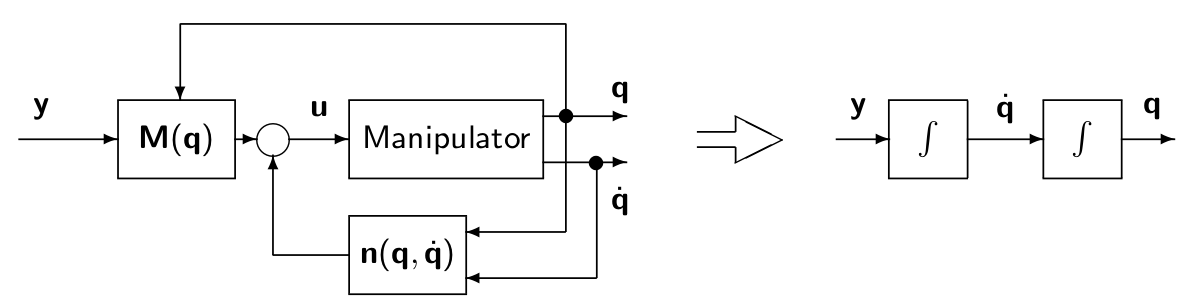
\includegraphics[width=\textwidth]{invkin}

The system results to be completely decoupled and linear. However, the resulting system has two poles in the origin and is therefore unstable. In order to stabilyze the system $y$ can be chosen as:
\[
    y= -K_D\dot{q}-K_Pq+r
\]
This means adding proportional and derivative control. From $\ddot{q}=y$ it follows:
\[
    \ddot{q}+K_D\dot{q}+K_Pq=r
\]
Which is asymptotically stable as long as $K_P$ and $K_D$ are positive-definite. If matrices $K_P,K_D$ are diagonal matrices defined by
\[
    K_P=diag\{\omega_n^2\} \qquad K_D=diag\{2\delta \omega_n\}
\]
the dynamics of the $i$-th component is characterized by the specified natural frequency and damping coefficient. A predefined trajectory $q_d(t)$ can be tracked by defining
\[
    r = \ddot{q}_d+K_D\dot{q}_d+K_Pq_d
\]
Then the dynamics of the tracking error is
\[
    \ddot{\tilde{q}} + K_D\dot{\tilde{q}} + K_P\tilde{q} = 0
\]
which converges to zero.
% TODO [insert image of control scheme]









\chapter{Advanced Position Control Schemes}









\section{Robust Control}
Aims at compensating directly possible errors deriving from model errors and/or external disturbances. Some of the most known robust control techniques:
\begin{itemize}
    \item H-infinity loop shaping
    \item Loop transfer recovery (LQG,LTR)
    \item Sliding mode control (SMC), a variation of variable structure control (VSS)
\end{itemize}
\subsection{Variable Structure Control}
\subsubsection{Example}
Consider a second order dynamic system described by 
\[
    \ddot{x}=-\psi x \quad \text{with } \quad \psi\in \{a_1^2,a_2^2\} \quad (a_1^2>1>a_2^2)
\]
% TODO [insert phase plane images slide 10]
Assuming that $\psi$ is a control input, by using the commutation law:
\[
    \psi=\begin{cases}
        a_1^2 \text{ if } x\dot{x}>0\\
        a_2^2 \text{ if } x\dot{x}<0\\
    \end{cases}
\]
An asymptotically stable system is obtained
% TODO [insert image from slide 10]
\subsubsection{Example}
Consider the system
\[
    \ddot{x}-\xi \dot{x}+\psi x = 0 \quad \xi >0 
\]
where we choose
\[
    \psi = \begin{cases}
        -a \quad (A)\\
        a \quad (B)
    \end{cases}
\]
The system is unstable (different signed elements of the equation).

In case (A), there are two real eigenvales, given by:
\[
    \lambda_{1,2} = \displaystyle\frac{\xi}{2}\pm \sqrt{\displaystyle\frac{\xi^2}{4}+a}
\]
one is stable (negative) and one unstable (positive)

In case (B) there are complex conjugate eigenvalues with positive real part given that $a>\frac{\xi^2}{4}$. 
% TODO [insert phase portraits]
By choosing
\[
    \psi = \begin{cases}
        -a \quad \text{if} \quad xs<0 \quad (A)\\
        a \quad \text{if} \quad xs>0 \quad (B)
    \end{cases} \quad s = -cx +\dot{x}
\]
where
\[
    c=\frac{\xi}{2}-\sqrt{\frac{\xi^2}{4}+a}<0
\]
is the inclination of the line representing the stable mode in the (A) case. The resulting system is asympotitically stable.

This type of control scheme is called Variable structure control or Sliding Mode Control (as the system goes towards a stable mode and "slides" towards the origin) and can be generalized:

We define a \emph{Sliding Surface} $S(x)=0$ based on which we decide which one of two control laws is used:
\[
    u_c = \begin{cases}
        K_1(x) \quad \text{if} \quad S(x)>0\\
        K_2(x) \quad \text{if} \quad S(x)<0\\
    \end{cases}
\]
% TODO [insert image of control scheme slide 13]

Two steps are involved in the design of variable structure control:
\begin{itemize}
    \item choice of the sliding surface $S(x)$ so that the control system has the desired dynamic behaviour 
    \item choice of the control law $u_i$ $(i=1,\dots,m)$ in order to force the state on the sliding surface $S_i(x)$ even in case of parameter variations or external disturbances. 
\end{itemize}
\subsubsection{Example}
Let us consider the second order system
\[
    \ddot{y} + a\dot{y} + by = \psi +u \qquad G(s) = \displaystyle\frac{1}{s^2+as+b}
\]
where $u$ is the control and $\psi$ is an external disturbance, supposed to be bounded with bounded first order derivative
\[
    |\psi|<\Delta_0 \qquad |\dot{\psi}|<\Delta_1
\]

Choice of the sliding surface:
\[
    S(x) = \dot{y} + cy = 0 \quad \text{with} \quad x=(y,\dot{y})
\]
When the state $x=(y,\dot{y})\in S(x)=0$:
\begin{itemize}
    \item the dynamics of the controlled system is exponentially asymptotically stable \[
            \dot{y} = -cy \quad \implies \quad y(t) = y(0)e^{-ct}, \quad c>0
    \]
    \item the output of the system $y(t)$ goes to zero with a velocity that depends only the parameter "$c$", that is on the chosen sliding surface
    \item the behaviour of the controlled system does not depend neither on the external disturbance nor on changes in the parameters $a$ and $b$. (ROBUST)
\end{itemize}

Choice of the control: It is possible to prove that the discontinuous control law
\[
    u(t) = -K \sgn S(x)
\]
is able to force the state towards the sliding surface $S(x)=0$ as long as $K>\Delta_0$, with total disturbance rejection. This control can only take the state of the system to 0. Substituting $y$ and $\dot{y}$ with the tracking error: $x=(e,\dot{e})$, we can track a given trajectory with the chosen dynamics, with $e=y_d-y$. If $y_d\neq 0 $ the set point is to be considered another disturbance to the system as it is an exogenous input to the system, requiring $y_d \times G(0)$ control effort to be compensated. The lower bound on $K$ therefore becomes:
\[
    K>\Delta_0+y_dG(0)
\]

\subsubsection{Continuous time}
When the state $x$ is on the sliding surface $S(x)=0$, we have the \emph{ideal sliding mode}: 
\begin{itemize}
    \item the control action $u(t)$ commutes with infinite frequency
    \item the oscillation produced on the output variable $y(t)$ has a null amplitude
\end{itemize}
\subsubsection{Discrete time}
If the VS control law is implemented as a discrete-time system we have:
\begin{itemize}
    \item a finite commutation frequency
    \item a residual oscillation on the output variable $y(t)$ (\emph{chattering})
\end{itemize}
The amplitude of the residual oscillation is proportional to the sampling period $T$ and the value of $K$ of the control action
\[
    |y(t)|\leq KT
\]
Therefore, it is not possible to force the state "exactly" on the surface $S(x)=0$, but it is rather possible to keep it within a sufficiently small neighbourhood of it (\emph{discrete sliding mode})
\subsection{The chattering problem}
From a practical point of view, it is not possible to commute the control between the two values $u^+,u^-$ at an infinite frequency. Therefore, "oscillations" are generated in the controlled system (or in the actuator), typically in a frequency range within the system's bandwidth\footnote{if the control input is discontinuous, all the frequencies are excited and the natural frequencies of the system are necessarily excited}. Then, non modelled dynamics may be excited and undesired behaviours may be obtained. Some methods have been proposed to avoid this problem, among them:
\begin{itemize}
    \item Boundary layers
    \item DIC (Discrete Integral Control)
\end{itemize}
\subsubsection{Boundary Layers}
A region with proper amplitude is defined around the sliding surface; in this region, the control action is not discontinuous, but rather it changes in a continuous way, linealry proportional to the error.
% TODO [insert boundary layer images slide 32]
\subsubsection{DIC (Discrete Integral Control)}
Let us assme that the disturbance is bounded with bounded first derivative:
\[
    |\psi|<\Delta_0 \qquad |\dot{\psi}|<\Delta_1
\]
In addition to the standard VS control term ($-k \sgn S(x)$), two additional contributions are used: a term proportional to the error $-\lambda S(x)$ and one proportional to the integral of its sign
\[
    \begin{cases}
        u(t) = -\lambda S(x) -k\sgn S(x)-\tilde{\psi}(t)\\
        \dot{\tilde{\psi}} (t) = h \sgn S(x)
    \end{cases}
\]
It is possible to prove the following: \\
If the parameters $k,h$ and $\lambda$ of the control law are chosen such that:
\[
    k>0, \quad h>\Delta_1, \quad h\lambda k > \Delta_1^2(1-ln2)
\]
then the controlled system is globally asymptotically stable, and the state reaches the sliding surface $S(x)=0$ in a finite time.
Note that there is no lower bound on $k$, and it can therefore be chosen to be quite small to reduce the chattering effect. The lower bound on $h$, means that the implemented controller must be faster than the disturbance (have a higher derivative). 

The resulting controller is composed of a proportional, integral and a switching component. If the proportional part is not present, i.e. $\lambda = 0$, the control action is still able to sabilize the system, but only for "small" initial conditions. 

\subsection{Robust control of industrial manipulators}
In general, it is difficult to compensate exactly the dynamics of a robot manipulator. In practice, what we get is only a partial compensation. Let us consider the inverse dynamics control:
\[
    u=\hat{M}(q)y+\hat{n}(q,\dot{q})
\]
where $\hat{M}$ and $\hat{n}$ represent the known part of the dynamic model. In general, uncertainties may be expressed as 
\[
    \tilde{M}=\hat{M}-M \qquad \tilde{n} = \hat{n} - n
\]
By using the above equation, we have
\[
    M\ddot{q}+n=\hat{M}+\hat{n}
\]
Since matrix $M$ is invertible, we have (adding and subtracting $y$)
\begin{gather*}
    \ddot{q} = y + (M^{-1}\hat{M}-I)y+M^{-1}\tilde{n}\\
    =y-\eta
\end{gather*}
with
\[
    \eta = (M^{-1}\hat{M}-I)y+M^{-1}\tilde{n}
\]
note that, if $\hat{M}=M$ and $\hat{n}=n$ then $\eta=0$ and $\ddot{q}=y$
By using the same control as in the ideal case:
\[
    y=\ddot{q}_d+K_D(\dot{q}_d-\dot{q})+K_P(q_d-q)
\]
The error dynamics $\tilde{q}$ is given by 
\[
    \ddot{\tilde{q}}+K_D\dot{\tilde{q}} + K_P\tilde{q}=\eta
\]
and it is therefore not possible to guarantee that $\tilde{q}$ goes to zero ($\eta$ depends on the uncertainties of the system)
From
\[
    \ddot{q}=y-\eta
\]
we have 
\[
    \ddot{\tilde{q}}=\ddot{q}_d-y+\eta
\]
Therefore, by defining $\xi = \begin{bmatrix}
    \tilde{q}^T  & \dot{\tilde{q}}^T
\end{bmatrix}^T $ as the state vector, we obtain the first order differential equation
\[
    \dot{\xi} = H\xi + D(\ddot{q}_d-y+\eta)
\]
with
\[
    H=\begin{bmatrix}
        0 & I \\ 0 & 0
    \end{bmatrix} \in \mathbb{R}^{2n\times 2n} \qquad D = \begin{bmatrix}
        0 \\ I
    \end{bmatrix} \in \mathbb{R}^{2n\times 2n}
\]
The problem with tracking a given trajectory ($q_d,\dot{q}_d,\ddot{q}_d$) may be solved by designing a control law $y$ that stabilizes the error dynamics $\xi$, that is nonlinear and time variant (because of $\eta$). Because of the properties of any assigned trajectory (boundedness of velocity/acceleration) and considering the properties of the dynamic model fo a robot manipulator(boundedness) it is possible to estimate the range of variablity of the uncertainties $\eta$ affecting the error dynamics. 

In order to compensate for the uncertainty term $\eta$, we define a control law as:
\[
    y = \ddot{q}_d +K_D\dot{\tilde{q}} + K_P\tilde{q}+w = \ddot{q}_d + w + \begin{bmatrix}
        K_P & K_D
    \end{bmatrix} \begin{bmatrix}
    \tilde{q} \\ \dot{\tilde{q}}
    \end{bmatrix}
\]
the error dynamics in this case results
\[
    \dot{\xi} = \tilde{H} \xi + D(\eta-w)
\]
where the eigenvalues of the matrix
\[
    \tilde{H}= (H-DK) = \begin{bmatrix}
        0 & I \\ -K_P & -K_D
    \end{bmatrix}
\]
have negative real part (as $K_P,K_D$ are positive definite)
By properly choosing the two matrices $K_P,K_D$ for example as 
\[
    K_P = diag\{\omega_{n1}^2,\dots,\omega_{nn}^2\} \qquad K_D = diag\{2\delta_1\omega_{n1},\dots,2\delta\omega_{nn}\} 
\]
it is possible to obtain a desired (and decoupled) behaviour for the linear part of the error dynamics. Notice that if $\eta=0$, then by choosing $w=0$ we obtain the previous control scheme. Viceversa, if $\eta\neq 0$, a proper value for $w$ must be defined. The Lyapunov method is adopted, choosing as a candidate Lyapunov function
\[
    V(\xi)=\xi^TQ\xi>0 \quad \forall \xi \neq 0
\]
where $Q$ is a symmetric, positive definite matrix
By derivation, since $\dot{\xi}=\tilde{H}\xi+D(\eta-w)$, we have:
\begin{gather*}
    \dot{V} = \dot{x}^TQ\xi+\xi^TQ\dot{x}\\
    =(\tilde{H}\xi+D(\eta-w)^TQ\xi+\xi^TQ/\tilde{H}\xi+D(\eta-w))\\
    =\xi^T(\tilde{H}^TQ+Q\tilde{H})\xi+2\xi^TQD(\eta-w)\\
    =-\xi^TP\xi+2\xi^TQD(\eta-w)\\
    =-\xi^TP\xi+2z^T(\eta-w)
\end{gather*}
where\[
    z=d^TQ\xi
\]
and, since $\tilde{H}<0$, the equation 
\[
    \tilde{H}^TQ+Q\tilde{H}=-P, \quad \forall P>0
\]
has a unique solution $Q$, symmetric and positive definite. 
Notice that the first term is negative definite. We need to prove negativity of the second term. The vector $z$ is known, therefore we can choose the control input:
\[
    w=\displaystyle\frac{\rho}{\|z\|}z \quad \rho>\|\eta\|
\]
we obtain
\begin{gather*}
    z^T(\eta-w)=z^T\eta-\displaystyle\frac{\rho}{\|z\|}z^Tz \leq \|z\|\|\eta\|-\rho\|z\| \leq 0
\end{gather*}
and thus
\[
    \dot{V}<0
\]
Overall control scheme:
% [TODO] insert image slide 52
This is akin to sliding mode control as the direction of $z$ cannot be assumed to be continuous. The sliding subspace $S(\xi)=D^TQ\xi=0$ depends on the choice of the matrix $Q$. The chattering problem may be solved e.g. by the 'boundary layers' method:
\[
    w=\begin{cases}
        \displaystyle\frac{\rho}{\|z\|}z \quad \text{when }\|z\|\geq\epsilon\\
        \displaystyle\frac{\rho}{\epsilon}z \quad \text{when }\|z\|<\epsilon
    \end{cases}
\]
Discrete Integral Control may exhibit some unexpected behaviour and implementative challenges due to the complexity of the system. 


\section{Adaptive Control}
Aims at modifying the control parameters in order to adapt to different working conditions, or to different values of the model parameters.
There are two main families of adaptive controllers:
\begin{itemize}
    \item Self Tuning Regulator (indirect)
    \item Implicit regulator (direct)
\end{itemize}
% [TODO] insert schemes slide 56
We assume the dynamics of the process to be linear wrt the parameters to be estimated, and we require the change of parameters to be slower than the dynamics of the system. 
\subsection{Robot parameters}
For design purposes:
\begin{itemize}
    \item kinematic parameters are assumed to be known (DH parameters, 3 per link)
    \item uncertain (constant) parameters that can be identified off line: masses(1), positions of CoMs(3), inertia matrices(6) (10 per link)
    \item parameters that are (slowly) varying during operation: viscous, dry and stiction friction at each joint (3 per joint)
    \item uknown and abruptly changing parameters: mass, CoM, inertia matrix of the payload wrt the tool center point (10)
\end{itemize}
so for an n-dof robot: $(3+10+3)\times n +10=16\times n +10 $ parameters

The main goals of an adaptive control scheme may be defined as:
\begin{itemize}
    \item given a twice differentiable desired joint trajectory $q_d(t),\dot{q}_d(t),\ddot{q}_d(t)$ 
    \item execute this trajectory under large dynamic uncertainties $\tilde{\alpha}=\alpha-\hat{\alpha}$ with a tracking error that vanishes asymptotically: \[
            \tilde{q}=q_d-q\to 0,\quad \dot{\tilde{q}}=\dot{q}_d-\dot{q}\to 0
    \]
    guaranteeing global stability
    \item paramenter identification (i.e. $\tilde{\alpha}\to 0$) is not of particular concern. 
        If the desired trajectory is persistently exciting, one obtaines parameter identification as a by-product ($\tilde{\alpha}\to 0$)
    \item indirect adaptive control schemes are more complex, but in principle allow also systematic convergence of dynamic coefficients to their true values
\end{itemize}
It is always possible to write the Euler-Lagrange formulation of the dynamics of an $n$ dof robot as 
\[
    Y(q,\dot{q},\ddot{q})\alpha = u
\]
where:
\begin{itemize}
    \item vector $\alpha$ contains only uknown or uncertain coefficients
    \item each component of $\alpha$ is in general a combination of the robot physical parameters
    \item the model regression matrix $Y$ depends: linearly on $\ddot{q}$, quadratically on $\dot{q}$, nonlinearly on $q$
\end{itemize}
In general, only a partial knowledge of the dynamic parameters is available, and therefore we may describe the dynamics of a robot as:
\[
    \hat{M}(q)\ddot{q}+\hat{C}(q,\dot{q})\dot{q}+\hat{D}\dot{q}+\hat{g}(q)=Y(q,\dot{q},\ddot{q})\alpha=u
\]
where $\hat{M},\hat{C},\hat{D},\hat{g}$ estimate $\alpha$.
Some controllers are better suited to adaptive control with robot manipulators.
\subsection{Inverse dynamics feedforward + PD}
% [TODO] insert inverse dynamics ff+PD scheme slide 66
Given a desired trajectory it is possible to implement an inverse dynamics ff + PD control action defined as:
\[
    u=M(q_d)\ddot{q_d}+C(q_d,\dot{q}_d)\dot{q}_d+D\dot{q}_d+g(q_d)+K_P\tilde{q}+K_d\dot{\tilde{q}}
\]
being $\tilde{q}$ and $\dot{\tilde{q}}$ the position and velocity errors. Since the dynamic parameters are in general not exactly known, only an approximation of the ff term can be computed. It can be shown that the control law leads to an error dynamics described by 
\[
    \ddot{\tilde{q}}+K_d\dot{\tilde{q}}+K_P\tilde{q}=\eta
\]
being $\eta$ a nonlinear function of the parameter uncertainties and of the nl dynamics of the robot, so the error does not vanish asymptotically
\subsection{NL control based on fb linearization}

The error dynamics behaves analogously to the previous case, and does not vanish asymptotically. 
\subsection{Nonlinear tracking control law without cancelations}
Let us consider a candidate control law:
\[
    u=M(q)\ddot{q}_d+C(q,\dot{q})\dot{q}_d+D\dot{q}_d+g(q)+K_p\tilde{q}+K_d\dot{\tilde{q}}
\]
that is a nonlinear trajectory tracking control law having global asymptotic stabilization properties. In principle, the control law could be made adaptive by defining 
\[
    \dot{\hat{\alpha}}=\gamma(\hat{\alpha},q,\dot{q},q_d,\dot{q}_d)
\]
where $\gamma(\cdot)$ is a proper update law for the robot's parameters

It can be shown that with this control law the velocities could track the desired ones (eventually with zero error), but a permanent residual position error may occur if parameters are not exactly known. A possible solution is to modify the velocity reference as 
\[
    \dot{q}_d \to \dot{q}_r=\dot{q}_d+ \Lambda(q_d-q), \quad \Lambda>0 
\]
where ofthe the value $\Lambda=K_d^{-1}K_p$ is chosen

In robotics, in order to design an adaptive control law we exploit the property of the dynamic model to be linear wrt the parameters 
\[
    Y(q,\dot{q},\ddot{q})\alpha=u
\]
Let us consider the control law:
\[
    u=M(q)\ddot{q}_r+C(q,\dot{q})\dot{q}_r+D\dot{q}_r+g(q)+K_D\sigma
\]
where 
\begin{flalign*}
    \dot{q}_r = \dot{q}_d+\Lambda\tilde{q}\\
    \ddot{q}_r = \ddot{q}_d+\Lambda\dot{\tilde{q}}
\end{flalign*}
and $K_D$ a positive definite matrix. The term $K_D\sigma$ is equivalent to a PD control action on the tracking error assuming 
\[
    \sigma=\dot{q}_r-\dot{q}=\dot{\tilde{q}}+\Lambda\tilde{q}
\]
The overall dynamics is the described by 
\[
    M(q) \dot{\sigma} +C(q,\dot{q})\sigma+D\sigma+K_D\sigma=0
\]

To prove stability of the system we use the Lyapunov method. We choose as a candidate Lyapunov function 
\[
    V(\sigma,\tilde{q}) = \displaystyle\frac{1}{2}\sigma^TM(q)\sigma+\displaystyle\frac{1}{2}\tilde{q}^TA\tilde{q}>0 \quad \forall \sigma,\tilde{q} \neq 0 
\]
where $A$ is positive definite.
The time derivative of $V$ is 
\begin{gather*}
    \dot{V}=\sigma^TM(q)\dot{\sigma}+\displaystyle\frac{1}{2}\sigma^T\dot{M}(q)\sigma+\tilde{q}^TA\dot{\tilde{q}}\\
    =\sigma^T[-C\sigma-D\sigma-K_D\sigma]+\displaystyle\frac{1}{2}\sigma^T\dot{M}\sigma+\tilde{q}^TA\dot{\tilde{q}}\\
    =\displaystyle\frac{1}{2}\sigma^T(\dot{M}-2C)\sigma-\sigma^TD\sigma-\sigma^TK_D\sigma+\tilde{q}^TA\dot{\tilde{q}} \qquad \sigma=\dot{\tilde{q}}+\Lambda\tilde{q} \\
    =-\sigma^TD\sigma-(\dot{\tilde{q}}+\Lambda\tilde{q})^TK_D(\dot{\tilde{q}}+\Lambda\tilde{q})+\tilde{q}^TA\dot{\tilde{q}} \qquad A=2\Lambda K_D\\
    =-\sigma^TD\sigma-\dot{\tilde{q}}^TK_D\dot{\tilde{q}}-\tilde{q}^T\Lambda K_D \Lambda \tilde{q}<0
\end{gather*}
Therefore $\dot{V}<0$, and $\dot{V}=0$ only when $\tilde{q}=\dot{\tilde{q}}\equiv 0$ $\implies$ $[\tilde{q}^T,\sigma^T]^T=0$ is GAS. The system evolves on $\sigma=0$ without a high.frequency control action.

On the basis of the previous result, let us consider the control law 
\[
    u = \hat{M}(q)\ddot{q}_r+\hat{C}(q,\dot{q})\dot{q}_r+\hat{D}\dot{q}_r+\hat{g}(q)+K_D\sigma = Y(q,\dot{q},\dot{q}_r,\ddot{q}_r)\hat{\alpha}+K_D\sigma
\]
computed using the estimation $\hat{\alpha}$ of the parameters of the dynamic model.
Notice that $Y$ does not depend on $\ddot{q}$. 
With this control, the overall dynamics are described by:
\begin{gather*}
    M(q)\dot{\sigma}+C(q,\dot{q})\sigma+D\sigma+K_D\sigma=-\tilde{M}(q)\ddot{q}_r-\tilde{C}(q,\dot{q})\dot{q}_r-\tilde{D}\dot{q}_r-\tilde{g}(q)\\
    =-Y(q,\dot{q},\dot{q}_r,\ddot{q}_r)\tilde{\alpha}
\end{gather*}
where
\[
    \tilde{M}=\hat{M}-M, \qquad \tilde{C}=\hat{C}-C, \qquad \tilde{g}=\hat{g}-g, \qquad \tilde{g}=\hat{g}-g, \qquad \tilde{\alpha}=\hat{\alpha}-\alpha 
\]
In order to prove the stability of the system under this new control law, we once again use the Lyapunov method: 
\[
    V(\sigma,\tilde{q},\tilde{\alpha})=\displaystyle\frac{1}{2}\sigma^TM(q)\sigma+\tilde{q}^T\Lambda K_D\tilde{q}+\displaystyle\frac{1}{2}\tilde{\alpha}^TK_\alpha \tilde{\alpha}>0 \qquad \forall \sigma,\tilde{q},\tilde{\alpha}\neq 0
\]
Where $K_\sigma$ is a symmetric positive definite matrix. It can be shown that the time derivative of $V$ is now : 
\[
    \dot{V}=-\sigma^TD\sigma-\dot{\tilde{q}}^TK_D\dot{\tilde{q}}-\tilde{q}^T\Lambda K_D \Lambda\tilde{q} + \tilde{\alpha}^T(K_\alpha\dot{\tilde{\alpha}}-Y^T(q,\dot{q},\dot{q}_r,\ddot{q}_r)\sigma)
\]
The function $\dot{V}$ is negative if the parameters are "adapted" according to 
\[
    \dot{\hat{\alpha}}=K_\alpha^{-1}Y^T(q,\dot{q},\dot{q}_r,\ddot{q}_r)\sigma
\]
As a matter of fact, we have 
\[
    \dot{V}=-\sigma^TD\sigma-\dot{\tilde{q}}^TK_D\dot{\tilde{q}}-\tilde{q}^T\Lambda K_D\Lambda\tilde{q}<0
\]
Therefore, with the control law 
\[
    u=Y(q,\dot{q},\dot{q}_r,\ddot{q}_r)\hat{\alpha}+K_d(\dot{\tilde{q}}+\Lambda\tilde{q})
\]
where the parameters are computed according to 
\[
    \dot{\hat{\alpha}}=K_\alpha^{-1}Y^T(q,\dot{q},\dot{q}_r,\ddot{q}_r)\sigma
\]
The overall dynamics converges to 
\[
    \sigma=0,\quad \tilde{q}=0 \quad (\dot{\tilde{q}}=0)
\]
and then $\tilde{q},\dot{\tilde{q}}$ converge to zero and moreover $\hat{\alpha}$ is bounded. Notice that from 
\[
    M(q)\dot{\sigma}+C(q,\dot{q})\sigma+D\sigma+K_D\sigma=- Y(q,\dot{q},\dot{q}_r,\ddot{q}_r)\tilde{\alpha}
\]
in steady state ($\dot{\sigma}=\sigma=0$) we have 
\[
    Y(q,\dot{q},\dot{q}_r,\ddot{q}_r)(\hat{\alpha}-\alpha)=0\quad \notimplies \quad \hat{\alpha}\to\alpha
\]
It is not possible to conclude that $\hat{\alpha}=\alpha$, but only that $\tilde{\alpha}\in Null\{Y\}$
The overall control scheme is 

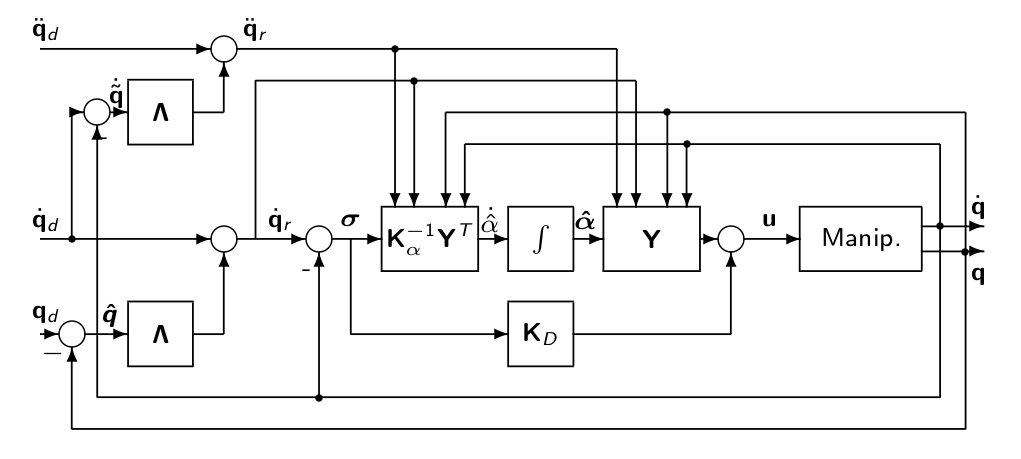
\includegraphics[width=\textwidth]{adapctrl}

This is an implicit adaptive control. There are three contributions: 
\begin{enumerate}
    \item term $Y\hat{\alpha}$, a control action similar to the inverse dynamics approach 
        \item term $K_D\sigma$, PD stabilizing action 
        \item estimated parameter vector $\hat{\alpha}$, updated according to a \emph{gradient} method, matrix $K_\alpha$ defines the speed of convergence of the estimated parameters.
\end{enumerate}
% slide 81 skipped 
\subsubsection{To sum up}

Adaptive control:
\begin{itemize}
    \item does not compensate directly external disturbance
    \item depends on the considered model 
    \item tries to compensate the effects of disturbances by modifying the parameters 
    \item "smooth" control action
\end{itemize}

Robust Control:
\begin{itemize}
    \item direct compensation of disturbances 
    \item chattering phenomenon
\end{itemize}







\chapter{Learning/Repetitive Control}
If a robot has to repeat a given task cyclically, following the same trajectory every time, possible uncertainties in the system may be compensated by adopting learning or repetitive control schemes, by means of which the contrl system, by repeating the task, learns the optimal control input to be applied in order to have zero tracking error. There are learning or repetitive control schemes to solve 
\begin{itemize}
    \item trajectory tracking problems 
    \item control to steady state configurations.
\end{itemize}
% [TODO] insert ff control scheme slide 4 
Two control actions: 
\begin{itemize}
    \item feedback, based on the error $e=y_d-y$ 
    \item feedforward, updated at each iteration
\end{itemize}


\section{PD control without gravity compensation}
Let us consider the following case:
\begin{itemize}
    \item Control to arbitrary constant (equilibrium) configuration of a robot subject to gravity \begin{itemize}
            \item without explicit knowledge of the dynamic coefficients and of the gravity term
            \item without using "high gain" position control terms
        \end{itemize}
    \item Use of an iterative control scheme based on \begin{enumerate}
            \item PD control on the joint position error + constant compensation (ff) term 
            \item iterative update of the ff term at each steady-state intermediate condition
        \end{enumerate}
\end{itemize}
Assumptions: 
\begin{itemize}
    \item dynamic model of the robot \[
            M(q)\ddot{q}+C(q,\dot{q})\dot{q}+g(q)=u
        \]
    \item boundedness of the gradient of the gravity term \[
            \|\displaystyle\frac{\partial g}{\partial q}\| \leq \alpha
        \] 
    \item joint-based PD controller (without g compensation) \[
            u= K_p(q_d-q) -K_d\dot{q} \quad K_p>0,K_d> 0
        \]
    \item it can be shown that the systeem is stable and that in steady-state we have:\[
            q=\bar{q},\quad \dot{q}=0,\quad g(\bar{q})=K_p(q_d-\bar{q}),\quad \tilde{q}=q_d-\bar{q}
        \]
\end{itemize}
Control scheme:
\begin{itemize}
    \item at the $i-th$ iteration, the control action is \[
            u(t) =\displaystyle\frac{1}{\beta}K_p(q_d-q(t))-K_d\dot{q}(t)+u_{i-1} \quad \beta>0,\quad q(0)=\bar{q}_{i-1}
            \] where \begin{itemize}
            \item the term $u_{i-1}$ is a proper, constant ff action 
            \item $u_0=0$ is the usual initial value 
            \item $q_0$ is the initial robot configuration
        \end{itemize}
    \item at the steady-state of the i-th iteration we have 
        \[
            g(\bar{q}_i) = \displaystyle\frac{1}{\beta} K_p(q_d-\bar{q}_i)+u_{i-1}
        \]
        \item the ff action (for the next iteration) is updated as 
            \[
                u_i = \displaystyle\frac{1}{\beta}K_p(q_d-\bar{q}_i)+u_{i-1} \quad (=g(\bar{q}_i))
            \]
\end{itemize}
\subsubsection{Theorem (sufficient condition for convergence)}
If the following conditions:
\begin{enumerate}
    \item $\lambda_{min}(K_p)\geq \alpha$
    \item  $0<\beta\leq 0.5$
\end{enumerate}
hold, then the sequence $\{q_0,\bar{q}_1,\bar{q}_2,\dots\}$ converges to $q_d$ from any initial condition ($q_0,\dot{q}_0$) (\emph{global convergence})
Condition (1) is sufficient for guaranteeing the global asymptotic stability (a unique equilibrium point exists for the closed loop system) with the control law. The additional sufficient condition (2) guarantees the convergence of the iterative scheme and in particular that 
\[
    \lim_{i\to\infty} u_i = g(q_d)
\]
\subsubsection{Proof}
Define $\tilde{q}=q_d-q$. At the end of each iteration, because of the update law, we have $u_i=g(\bar{q}_i)$ and therefore 
\[
    \|u_i-u_{i-1}\| = \| g(\bar{q}_i)-g(\bar{q}_{i-1}) \| \leq \alpha\|\bar{q}_i-\bar{q}_{i-1}\| \leq \alpha(\|\tilde{q}_i\| + \|\tilde{q}_{i-1}\|)
\]
from the update law we have 
\[
    \|u_i-u_{i-1}\| = \displaystyle\frac{1}{\beta}\|K_p\tilde{q}_i\|
\]
By combining the above relations, and taking advantage of condition 1. we get 
\[
    \displaystyle\frac{1}{\beta}\alpha \|\tilde{q}_i\| \leq \displaystyle\frac{1}{\beta}\lambda_{min}(K_p)\|\tilde{q}_i\| \leq \displaystyle\frac{1}{\beta}\|K_p\tilde{q}_i\| \leq \alpha(\|\tilde{q}_i\|+\|\tilde{q}_{i-1}\|)
\]
which means that 
\[
    \displaystyle\frac{1}{\beta} \|\tilde{q}_i\| \leq (\|\tilde{q}_i\|+\|\tilde{q}_{i-1}\|)
\]
which can be rewritten as 
\[
    \|\tilde{q}_i\| < \displaystyle\frac{\beta}{1-\beta}\|\tilde{q}_{i-1}\|
\]
which because of condition 2 is a contraction mapping, and therefore 
\[
    \lim_{i\to\infty} \|\tilde{q}_i\|=0
\]
with asymptotic convergence from any initial condition. 
\subsubsection{comments}
\begin{itemize}
    \item By sobstitution of condtions 1. and 2. in the control law, we have that the matrix defining the proportional gains becomes 
        \[
            \hat{K}_p=K_p/\beta \implies \lambda_{min}(\hat{K}_p)>2\alpha
        \]
    \item if $K_p$ is a diagonal matrix, this condition implies a lower bound for each element of the diagonal 
    \item It is a sufficient condition: the scheme could converge even if it is not satisfied 
    \item The overall scheme can be interpreted as a control law with an integral action updated in correspondence of a discrete sequence of time instants (each steady state), achieving GAS
\end{itemize}
\subsection{Final comments}
\begin{itemize}
    \item convergence is achieved in few iterations 
    \item  the condition on the proportional gain is sufficient: the system might converge even if it is violated 
    \item it is possible, with a more detailed analysis to determine lower bounds on the gains $K_{p,j}$ with a smaller value but still sufficient to guarantee stability 
    \item it is reasonable to assume that these values are lower for the distal links of the robot 
    \item in practical cases, the update of the control law is performed the robot is sufficiently close to a steady state condition 
    \item this approach has been extended to the case of flexible (joints and/or links) robot arms
\end{itemize}


\section{Repetitive control}
\subsection{Internal Model Principle}
Accurate control can be achieved only if the control system encapsulates (either implicitly or explicitly) some representation of the process to be controlled. 

Once the controlled system contains an internal model of the signal to be tracked, and \emph{the overall system is stabilized}, perfect tracking is achieved. 
\subsection{Fourier Decomposition and IMP}
Since our initial hypothesis states that we have to deal with periodic reference signals of known period $\tau$, let's see how these signals can be modelled and how we can connect them with the IMP idea: 

The Fourier Decomposition Theorem states that any periodic function (or periodic signal) can be decomposed into the sum of a (possibly infinite) set of simple oscillating functions represented by sines and cosines. 

In particular, we can express a periodic reference signal $y_{ref}(t)$ with period $\tau$ as 
\[
    y_{ref}(t) = \displaystyle\sum_{k=0}^{\infty}A_ksin(k\omega_\tau+\phi_k) \quad \text{with} \quad \omega_\tau=\displaystyle\frac{2\pi}{\tau}
\]
In general, in most control applications we deal with (well known) simple signals. Therefore, we assume that the model of any of these (periodic) functions is knwon and represented by a pair of poles on the imaginary axis 
\[
    \displaystyle\frac{1}{s^2+(k\omega_\tau)^2} \longrightarrow s = \pm jk\omega_\tau
\]
According to the IMP, if any of these modes (coming from the Fourier Decomposition of the periodic reference) is embedded in the control system, perfect tracking will be achieved by the control system. In practice we need a system that acts as internal model for any periodic signal of period $\tau$, thus a system having infinitely many poles on the imaginary axis at multiple integers of $\omega_\tau$.
The transfer function of such a system can be represented as 
\[
    \displaystyle\frac{1}{s\prod_{k=1}^\infty (s^2+k^2\omega_\tau^2)}
\]
A system with this dynamic characterization is called \emph{Repetitive Compensator} and represents the core of any RC system. Let us consider the following scheme: 
% [TODO] insert scheme slide 17 
It generates any periodic signal of period $\tau$ (with a suitable initial function stored in the delay block). It works as the internal model for periodic signals of period $\tau$. The pure delay present in the positive feedback loop implements the dynamic system with the desired poles on the imaginary axis. 

The repetitive compensator presents a closed loop trasnfer function 
\[
    \displaystyle\frac{e^{-\tau s}}{1-e^{-\tau s}}
\]
The poles of this system are those complex numbers such that 
\[
    e^{-\tau s} = 1 
\]
By setting $s = \sigma+j\omega$ it results 
\[
    e^{-\tau\sigma} e ^{-j \omega \tau} = 1 = e^{j2k\pi}
\]
from which 
\begin{gather*}
    \sigma = 0 \\
    \omega = \displaystyle\frac{2k\pi}{\tau} = k \omega_\tau, \quad k \text{ integer}
\end{gather*}
Thus exactly the infinite number of poles palced where needed. This proves that the repetitive compensator acts as internal model for any periodic signal of period $\tau$. Stability analysis is necessary to evaluate the functionality of the scheme. 

\subsection{Nyquist-Driven Stability Analysis}
In order to analyse the stabilty properties, we can consider the following system which has the same characteristic equations (and consequently the same poles) of the previous one. As a matter of fact, the overall transfer fucntion is given by 
\[
    G_0(s) = \displaystyle\frac{e^{-\tau s}(P(s)) }{1+e^{-\tau s}(P(s)-1)}
\]
and therefore, the characteristic equation is 
\[
    1+e^{-\tau s}(P(s)-1)=0
\]
In order to analyse the stability properties, we can consider the following system which has the same characteristic equations (and consequently the same poles) of the previous one
with the same characteristic equation as $G_0(s)$ 
\[
    H_0(s) = \displaystyle\frac{e^{-\tau s}(P(s)-1) }{1+e^{-\tau s(P(s)-1)}}
\]
\subsubsection{Nyquist Stability Criterion} 
The Nyquist Stability Criterion is a very effective tool to determine whether a closed loop system is stable or not without computing explicitly the closed loop poles of the system, i.e. the roots of $1+L(s)=0$

The criterion states that the closed loop system with open loop tf $L(s)$ (stable), is stable iff the polar plot of $L(jw)$ does not encircle or touch the critical point $-1$ on the complex plane. 
\begin{itemize}
    \item The polar plot can be constructed by evaluating on the complex plane the image of $L(jw)$ parametrized for $w$ ranging from 0 to $+\infty$ and then closing the plot in a specular way about the real axis 
    \item the overall plot will always form a closed curve because it derives from a mapping that has a closd curve as domain (called \emph{Nyquist Path}) 
    \item The Nyquist path is a curve that has as interior the whole right half plane 
\end{itemize}
If the loop transfer function is not rational but contains some delay term it is still worth to apply the Nyquist criterion for stability analysis of the closed loop systems. Let us consider a system with loop transfer function 
\[
    L(s) = e^{-\delta s} L'(s)
\]
The greater the value of the delay $\delta$, the greater the negative phase shift. This behaviour can easily cause instability in the closed loop system. The polar plot of such a system presents rotational behaviour with increasing speed with growing values of $\omega$. A very important corollary of the Nyquist criterion that will be used in the following states that a sufficient condition for stability of the closed loop system is 
\[
    |L(j\omega)|<1 \quad \forall \omega
\]
By applying the Nyquist Criterion to the RC scheme, it follows that a sufficient condition for stability of the RC scheme is 
\[
    \|P(j\omega)-1\| < 1 \quad \forall \omega
\]
This condition is never satisfied unless P is biproper (rel degree 0). However, it requires too much: tracking arbitrary periodic signals (even discontinuous ones).
\subsubsection{Possible Remedies}
The nonexistence of a repetitive controller for a strictly proper pant is not surprsing: if $P(s)$ has non null relative degee it "integrates" the input at least once, and hence the output will be smoothed out to some extent making it impossible to track a signal with an infintely sharp edge. To overcome this problem two solutions have been found:
\begin{enumerate}
    \item Introduction of a filter in the delay (often called Modified Repetitive Control Scheme)
    \item Make it a discrete time system, that provides a natural upper bound to the maximum meaningful frequency value 
\end{enumerate}
\subsection{Modified Repetitive Control System}
The modified RC system presents a low-pass filter Q(s) that multiplies the pure delay in the repetitive compensator. 
\begin{itemize}
    \item Exact internal model is lost: the repetitive compensator acts as internal model for any periodic signal of period $\tau$ within a certain frequency range 
    \item problems in high frequency tracking 
    \item the poles escape away from the imaginary axis for high values of $\omega$ 
\end{itemize}

\subsection{Discrete Time Repetitive Control}
The most commonly adopted solution is to make the system a digital system. Any periodic signal with period N (N samples) can be generated by an \emph{N-step delay with positive feedback loop}. This means that such a system must represent the repetitive compensator in discrete time version. We can interpret the complex function $z^{-1}$ as the one-step delay operator. 
% what are you doing step-delay?

The discrete time repetitive compensator has a closed loop transfer function 
\[
    \displaystyle\frac{z^{-N}}{1-z^{-N}}
\]
the poles of this system are those complex numbers such that $z^{-N}=1$. By setting $z=\rho e^{-j\theta N}$ it results 
\[
    \rho e^{j\theta N} = 1 = e^{j2k\pi}
\]
from which 
\begin{align*}
    \rho = 1 \\
    \theta = \displaystyle\frac{2k\pi}{N}, \quad k \text{ integer}
\end{align*}
Thus exactly N poles on the unit circle in the z-plane. In discrete time signal analysis these poles represent the simple oscillation modes whose linear combination can produce any periodic signal of period N (Discrete Fourier Decomposition). This proves that the discrete time repetitive compensator acts as internal model for any periodic signal of period N. 
Note that tracking is only achievable at the sample points. 

Repetitive Control applied in a nonlinear system framework has been studied and in some cases satisfactory results have been achieved. Since in most industrial robotics applications cyclic operations are needed, RC can be a robust solution for the accomplishment of these tasks considering the lack of knowledge of the parameters can be seen as a periodic disturbance as the reference is periodic. 


\chapter{Force Control}
Force control is rather difficult whith very stiff objects, therefore it is appropriate to introduce some compliance between the robot and the environment. 
\section{Passive Compliance}
Mechanical devices properly installed on the wrist of the robot, able to react to external forces (RCC: Remote Center of Compliance)
\begin{itemize}
    \item advantages: low cost, simple devices
    \item low flexibility, use limited to specific applications
\end{itemize}
The center of compliance is a point in space where linear forces correspond to pure linear displacements and torques correspond to pure rotation.
% [TODO] insert images from slides


\section{Active Compliance}
Achieved by means of suitable control laws: the robot reacts in a programmed manner to external forces applied to the end-effector (a force sensor is usually required). 

\begin{itemize}
    \item advantages: high operational flexibility
    \item drawbacks: computational complexity, an environment model could be required
\end{itemize}

Different techniques are available: 
\begin{itemize}
    \item Pure force control: (theoretically) used in quasi-static applications 
    \item Active stiffness control: control of interaction forces is obtained on the basis of position control with an elastic model of the environment 
    \item Impedance control: a desired dynamic behaviour of the end-effector is imposed (mechanical impedance: ratio between force and velocity)
    \item Hybrid position/force control: the directions in the operational space are separated into position-controlled and force-controlled directions (on the basis of kinematic models of the task and of the dynamic model of the robot)
\end{itemize}

\subsection{Stiffness control}
Basic idea: \\
Force on the environment: $f_e = k_e(x-x_e)$\\
system dynamics: $m\ddot{x}+k_e(x-x_e)=f$
where $x_e$ is the original position of the contact point of the environment, and $x$ is the actual position of the contact. We choose to use a PD control:
\begin{gather*}
    m\ddot{x}+k_e(x-x_e)=f=k_p(x_d-x)-k_v\dot{x}\\
    m\ddot{x}+k_v\dot{x}+(k_p+k_e)x=k_px_d+k_ex_e
\end{gather*}
In steady state 
\[
    x=\displaystyle\frac{k_px_d+k_ex_e}{k_p+k_e}
\]
and then
\[
    f_e = k_e\left[\displaystyle\frac{k_px_d+k_ex_e}{k_p+k_e}-x_e\right] = \displaystyle\frac{k_e}{k_p+k_e}k_p(x_d-x_e)
\]
which is equivalent to two springs in series, a robot "spring" + and environment "spring"
\begin{itemize}
    \item if $k_e \gg k_p$ then $f_e\approx k_p(x_d-x_e)$ (compliant robot)
    \item if $k_p \gg k_e$ then $f_e\approx k_e(x_d-x_e)$ (compliant environment)
\end{itemize}
We obtain force control by means of position control. The stiffness of the system is defined by the gain $k_p$

Let us consider now a $n$ dof robot: Elastic environment:
\[
    w=\begin{bmatrix}
        f \\ n
    \end{bmatrix}= \begin{bmatrix}
    K_f & 0 \\ 0 & K_v
    \end{bmatrix}\begin{bmatrix}
        dp \\ \omega dt
    \end{bmatrix} = K\begin{bmatrix}
        dp \\ \omega dt
    \end{bmatrix}
\]
By using work-space coordinates (RPY,\dots)
\[
    w = KT_A(x)dx = KT_A(x)(x_e-x)
\]
With the analytic expression of the jacobian we have (from $J=T_AJ_A$ and $\tau=J^Tw=J_A^Tw_A$)
\[
    w_A=T_A^T(x)KT_A(x)dx=K_A(x)(x_e-x)
\]
$K_A$ is the (positive semi-definite) \emph{stiffness matrix}: the environment may not be able to generate forces along all the directions. Note that this matrix is not constant as it depends on the position $x$. In case it may be defined, $K_A^{-1}$ is the \emph{compliance matrix}. The range space of matrix $K_A$, i.e. $\mathcal{R}(K_A)$, defines the directions in the work space along which forces may be applied. \\
Dynamic model of the robot: 
\[M(q)\ddot{q}+C(q,\dot{q})\dot{q}+D\dot{q}+g(q)=u+J^T(q)w\] 
Control (PD+gravity compensation): 
\[u=g(q)+J_A^T(q)K_P\tilde{x}-J_A^T(q)K_DJ_A(q)\dot{q}\]
This control is obtained by transforming the standard PD+gravity control into the joint space by the analytic Jacobian. As velocities in the workspace are not measured, we make use of the equivalence $\dot{x}_A=J_A\dot{q}$.\\
In steady-state:
\[
    J_A^T(q)K_P\tilde{x}=-J^T(q)w \quad (=-J_A^T(q)w_A=-J_A^T(q)T_A^Tw)
\]
and, if the inverse of the Jacobian exists
\[
    \tilde{x}=-K_P^{-1}T_A^T(x)w = -K_P^{-1}w_A
\]
The compliance is defined by $K_P^{-1}$. If it is diagonal, the compliance referred to forces is linear and configuration-independent; this is not true for the torques due to the presence of $T_A$. 
We have
\[
    \tilde{x}=-K_P^{-1}K_A(x)(x_e-x)
\]
\subsubsection{Stiffness control in joint space}
Given the dynamic model in the joint space: 
\begin{gather*}
    M(q)\ddot{q}+C(q,\dot{q})\dot{q}+D\dot{q}+g(q)=u+J^T(q)w \\
    u=g(q)+K_P\tilde{q}-K_D\dot{q}
\end{gather*}
in steady state: 
\begin{gather*}
    K_P\tilde{q}=-J^Tw\\
    \tilde{q}=-K_p^{-1}J^Tw
\end{gather*}
under the assumption of small displacements we can consider 
\[
    \tilde{x}=J(q)\tilde{q}
\]
and therefore 
\begin{gather*}
    \tilde{x}=-J(q)K_P^{-1}J^T(q)w\\
    \tilde{x}=-J(q)K_P^{-1}J_A^T(q)w_A\\
    \tilde{x}=-J(q)K_P^{-1}J_A^T(q)K_A(x_e-x)
\end{gather*}
\subsection{Impedance control}
The goal is not to track specific desired position/velocity or force trajectories, but rather to define a dynamic relationship between velocities and forces. We define a desired work-space dynamics. We have:
\[
    \displaystyle\frac{w(s)}{\dot{x}(s)}=Z(s) \quad \text{or} \quad \displaystyle\frac{w(s)}{x(s)}=sZ(s)
\]
By defining
\[
    sZ(s)=-(M_ds^2+D_ds+K_d)
\]
where $M_d$ is the desired inertia matrix, $D_d$ is the desired damping and $K_d$ is the desired stiffness, we have
\[
    M_d\ddot{x}+D_d\dot{x}+K_dx=-w
\]
that defines the desired behaviour of the manipulator

We have a two-step design procedure:
\subsubsection{1) Linearization in the work-space}
\[
    \hat{M}(x)\ddot{x}+\hat{C}(x,\dot{x})\dot{x}+\hat{g}(x)=F+F_a
\]
where
\begin{gather*}
    \hat{M} = (JM^{-1}J^T)^{-1}=J^{-T}MJ^{-1}\\
    \hat{C} = \hat{M}(JM^{-1}CJ^{-1}-\dot{J}J^{-1})=J^{-T}CJ^{-1}-\hat{M}\dot{J}J^{-1}\\
    \hat{g} = \hat{M}JM^{-1}g = J^{-T}g
\end{gather*}
by defining 
\[
    F = [\hat{M}(x)y+\hat{C}(x,\dot{x})\dot{x}+\hat{g}(x)-F_a] = [\hat{M}(x)y+\hat{n}(x,\dot{x})-F_a]
\]
we obtain the linear model 
\[
    \ddot{x}=y
\]
\subsubsection{2) Definition of the desired impedance behaviour}
\[
    y=\ddot{x}_d+M_d^{-1}[D_d(\dot{x}_d-\dot{x})+K_d(x_d-x)+F_a]
\]
from which
\[
    M_d(\dot{x}_d-\ddot{x})+D_d)\dot{x}_d-\dot{x})+K_d(x_d-x)=-F_a
\]
or 
\[
    M_d\ddot{\tilde{x}}+D_d\dot{\tilde{x}}+K_d\tilde{x}=-F_a
\]
$F_a$ must be added because if it is not, the robot will go to $\tilde{x}=0$ ignoring external forces, leading to potential damage.
In conclusion, the overall control input $F$ is:
\[
    F = \hat{M}\ddot{x}_d +\hat{M}M_d^{-1}[D_d(\dot{x}_d-\dot{x})+K_d(x_d-x)+F_a]+\hat{n}(x,\dot{x})-F_a
\]
note that if we choose $M_d=\hat{M} (=J^{-T}MJ^{-1})$ then the control law is greatly simplified since 
\[
    F = \hat{M}\ddot{x}_d+[D_d(\dot{x}_d-\dot{x})+K_d(x_d-x)+F_a]+\hat{n}(x,\dot{x})
\]
and it does not even need a F/T sensor to be implemented. Since typically the control action is applied at the joint level, we have 
\[
    u=J^TF
\]
\subsubsection{Choice of the desired impedance}
The robot should:
\begin{itemize}
    \item avoid high impact forces due to uncertainties on position/shape of the environment 
    \item adapt to the stiffness properties of the environment 
    \item mimic a "human" behaviour: fast and rigid in free-space motion, slow and compliant during the approach and contact phases 
\end{itemize}
Then:
\begin{itemize}
    \item high values of $M_{d,i}$ and small values of $K_{d,i}$ along directions in the work space where contacts are expected 
    \item high values of $K_{d,j}$ and small values of $M_{d,j}$ along free directions in the work space (no contacts) 
    \item if the environment is stiff, small values of $K_{d,i}$ 
    \item the values of $D_{d,k}$ are used to modify the transient phases
\end{itemize}

\section{Hybrid position/force control}
When a task involves at the same time both motion and force application, it often happens that directions along which forces are applied are different with respect to directions along which motion takes place.

It is always possible to define, in a proper reference frame 
\begin{itemize}
    \item Natural constraints: directions along which the task gives constraints in position (velocity) and force 
    \item Artificial constraints: directions along which it is possible to assign desired constraints with the control system. 
\end{itemize}
These constraints are complementary and altogether define the 12 dofs of a given task: 6 dof in terms of position/velocity and 6 dof in terms of forces/torques. 

The artificial constraints define directions in the workspace along which it is possible to assign desired values of a given variable (velocity or force). It is then simple to design a "hybrid" control structure able to impose proper values along these directions only. 

Consider now the velocity domain $v$. Given the natural and artificial constraints, it is possble to decompose $v$ in two components:
\[
    v=v_a+v_n
\]
where the "free" directions (velocities) $v_a$ are complementary to the directions in $v_n$, that is 
\[
    v_a^Tv_n=0
\]
Note that the vectors cannot be said to be orthogonal as their norm cannot be defined, due to them being comprised of both linear and angular parts, leading to the vector space of the velocities $v$ not having a norm. Given a desired task, it is possible to define a base matrix $A_v$ that describes all the free velocities $v_a$:
\[
    A_v\in\mathbb{R}^{6\times n_a} \quad \text{such that} \quad v_a=A_vy 
\]
and a base matrix $N_v$ that describes all the remaining components 
\[
    N_v\in\mathbb{R}^{6\times 6-n_a} \quad \text{such that} \quad v_n=N_vy 
\]
with
\[
    A_v^TN_v=0    
\]
Given the matrix $A_v$, the goal is to control motions in $\mathcal{R}(A_v)$

Therefore, it is desired to control the components of a generic velocity vector $v$ satisfying 
\[
    A_v^Tv=A_v^TA_vy+A_vN_vz
\]
from which by setting $v_n=0$  
\[
    v_a = A_vy=A_v(A_v^TA_v)^{-1}A_v^Tv=\Sigma_vv
\]
Matrix $\Sigma_v$ is known as the \emph{selection matrix} and, if defined with respect to the contact reference frame, results a diagonal matrix with elements "1" and "0" on the diagonal\\
NB: $\Sigma_v$ is a projector matrix from $\mathbb{R}^6$ in $\mathcal{R}(A_v)$

Similarly, in the force domain it is possible to define a base matrix $A_f$ of the artificial contstrainsts, and the force components that it is possible to control are described by 
\[
    \Sigma_f=A_f(A_f^TA_f)^{-1}A_f^T
\]
In order to establish a Euclidean scalar product in the force/velocity vector spaces it is necessary to define specific metrics in these spaces. 
Once the selection matrices $\Sigma_v,\Sigma_f$ have been defined, it is possible to use these general control schemes: 
\begin{itemize}
    \item Control in joint space: 
        \begin{figure}[H]
            \begin{center}
                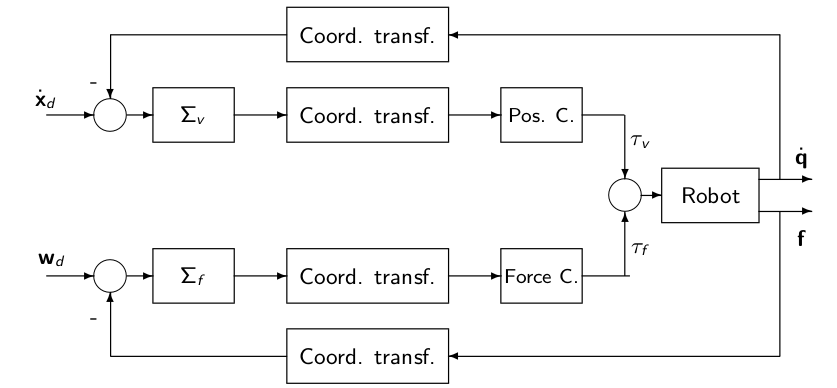
\includegraphics[width=0.95\textwidth]{hybridjspace}
            \end{center}
            \label{fig:}
        \end{figure}
    \item Control in work space 
        \begin{figure}[H]
            \begin{center}
                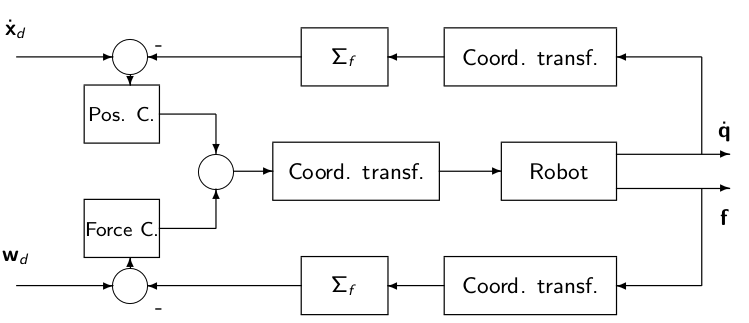
\includegraphics[width=0.95\textwidth]{hybridwspace}
            \end{center}
            \label{fig:}
        \end{figure}
\end{itemize}

\chapter{Trajectory planning for Robot Manipulation}
The planning modalities for trahectories may be quite different: 
\begin{itemize}
    \item point-to-point 
    \item with pre-defined path 
\end{itemize}
Or:
\begin{itemize}
    \item in the joint space
    \item  in the work space, either defining some points of interest (initial and final points, via points) or the whole geometric pat $x=x(t)$
\end{itemize}
For planning a desired trajectory, it is necessary to specify two aspects:
\begin{itemize}
    \item geometric path 
    \item motion law 
\end{itemize}
wiht constraints on the continuity of the trajectory and on its time derivatives up to a given degree. 

\subsection{Geometric path and motion law}
The geometric path can be defined in the work-space or in the joint-space. Usually, it is expressed in a parametric form as 
\begin{gather*}
    p=p(s) \qquad \text{work-space}\\
    q=q(\sigma)\qquad \text{joint-space}
\end{gather*}
Together, the geometric path and the motion law adefine the trajectory $p(s(t))$, or in short  $p=p(t)$. Note that, with the chain rule, 
\begin{gather*}
    \dot{p}=\displaystyle\frac{dp}{ds}\dot{s}\\
    \ddot{p}=\displaystyle\frac{dp}{ds}\ddot{s}+\displaystyle\frac{d^2p}{ds^2}\dot{s}^2
\end{gather*}
Input data to an algorithm for trajectory planning are: 
\begin{itemize}
    \item data defining the path 
    \item geometrical constraints on the path 
    \item constraints on the mechanical dynamics 
    \item constraints due to the actuation system 
\end{itemize}
Output: the trajectory in the joint or work-space, given as a sequence (in time) of the position, velocity and acceleration values. 
\subsubsection{1. Kinematic constraints}
Constraints on the minimum/maximum values for the derivatives up to a given order:
\[
    q^{(i)}_{min}\leq q^{(i)}\leq q_{max}^{(i)} \quad i=1,\dots,n
\]
in some cases $|q_{min}^{(i)}|\neq |q_{max}^{(i)}$
Constraints on torque may be "converted" into kinematic constraints. Cosntraining jerk physically means limiting vibrations. 
\subsubsection{2. Constraints on the order of continuity}
We have to choose a proper order $n$ of continuity for the motion law, i.e. 
\[
    q(t)\in C^n
\]
that is the $n$-th derivative $q^{(n)}(t)$ of function $q(t)$ is continuous, and $q^{(n+1)}(t)$ is composed of constant segments
\begin{itemize}
    \item the higher $n$, the "smoother" the profile: the frequency bandwidth will be reduced (better for vibration effects) 
    \item For control purposes (ff) the continuity of the trajectory should guarantee a limited control action 
    \item in high dynamics mechanical system, continuity of (at least) acceleration is required
\end{itemize}
\subsubsection{3. Dynamic consraints}
These constraints aim to reduce possible vibration effects on the mechanical load. 

\section{Joint-space trajectories}
Trajectories are specified by defining some characteristic points:
\begin{itemize}
    \item directly assigned by some specifications
    \item assigned by defining desired configurations $x$ in the woek-space, which are the converted in the joint-space using the inverse kinematic model.
\end{itemize}
The algorithm that computes a function $q(t)$ interpolating the given points is characterized by the following features:
\begin{itemize}
    \item trajectories must be computationally efficient 
    \item the position and velocity profiles must be continuous functions of time 
    \item undesired effects (such as non regular curvatures) must be minimized or completely avoided. 
\end{itemize}
Single joint trajectories may be classified as 
\begin{itemize}
    \item Polynomial trajectories 
    \item Trigonometric trajectories (cycloidal, harmonic)
    \item Trajectories based on Fourier series expansion 
    \item Composed trajectories (Trapezoidal velocity, double s, \dots)
    \item Spline (B-Splines, NURBS,\dots)
    \item Trajectories based on FIR (Finite Impulse Response) filters
\end{itemize}

\subsection{Polynomial trajectories}
In the most simple cases, a trajectoru is specified by assigning initial and final conditions on: time (duration), position, velocity, acceleration, \dots Then, the problem is to determine a function 
\[
    q=q(t) \quad \text{or} \quad q=q(\sigma), \quad \sigma=\sigma(t)
\]
so that those conditions are satisfied 

This is a boundary condition problem, that can be easily solved by considering polynomial functions such as: 
\[
    q(t)=a_0+a_1t+a_2t^2+\dots+a_nt^n
\]
The degree $n$ (3,5,\dots) of the polynomial depends on the number of boundary conditions that must be verified and on the desired "smoothness of the trajectory"

In general, besides the initial and final values, other constraints could be specified on the values of some time-derivatives in generic instans $t_j\in[t_i,t_f]$. In other terms, one could be interested in defining a polynomial function $q(t)$ whose $k$-th derivative has a specified value $q^k(t_j)$ at a given time instant $t_j$. Mathematically, these conditions are expressed as: 
\[
    k!a_k+(k+1)!a_{k+1}t_j+\dots+\displaystyle\frac{n!}{(n-k)!}a_nt_j^{n-k}=q^k(t_j)
\]
or, expressing all condiitions in matrix form: 
\[
    Ma=b
\]

\subsubsection{Third-order polynomial trajectories}
Given an initial and final instant, $t_i,t_f$, a trajectory may be specified by assigning initial and final conditions on: 
\begin{itemize}
    \item initial position and veloccity 
        \item final position and velocity 
\end{itemize}
There are four boundary conditions, and therefore a polynomial of degree (at least) 3 must be considered
\[
    q(t)=a_0+a_1t+a_2t^2+a_3t^3
\]
in order to solve these equations, let us assume for the time being that $t_i=0$. Therefore: 
\begin{gather*}
    a_0=q_i \\
    a_1  = \dot{q_i}\\
    a_2 = \displaystyle\frac{-3(q_i-q_f)-(2\dot{q}_i+\dot{q}_f)t_f}{t_f^2}\\
    a_2 = \displaystyle\frac{2(q_i-q_f)-(\dot{q}_i+\dot{q}_f)t_f}{t_f^3}
\end{gather*}
The results obtained can be generalized tot he case in whic $t_i\neq0$ :
\[
    q(t)=a_0+a_1(t-t_i)+a_2(t-t_i)^2+a_3(t-t_i)^3
\]
% [TODO] finish copying computations slide 35
Often, a trajectory is assigned by specifying a sequence of desired points (via-points)
without indication on the velocity in these points.
In these cases, the “most suitable” values for the velocities must be automatically
computed.
This assignment is quite simple with heuristic rules such as:
\begin{gather*}
    \dot{q}_1 = 0\\
    \dot{q}_k= \begin{cases}
        0 \quad sign(v_k)\neq sign(v_{k+1})\\
        \displaystyle\frac{1}{2}(v_k+v_k+1) \quad sign(v_k)=sign(v_k+1)
    \end{cases}\\
    \dot{q}_n=0
\end{gather*}
being 
\[
    v_k = \displaystyle\frac{q_k-q_{k-1}}{t_k-t_{k-1}}=\displaystyle\frac{K_k}{T_k}
\]
the slope of the $k$-th tract $\begin{bmatrix}
    t_k-1 & t_k
\end{bmatrix}$

\subsubsection{Fifth-order polynomial trajectories}
From the above examples, it may be noticed that both the position and velocity profiles are continuous functions of time. This is not true for acceleration, that presents discontinuities among different segments. Moreover, it is not possible to specify for this signal suitable initial/final values in each segment. In many applications, these aspects do not constitute a problem, being the trajectories "smooth" enough.  On the other hand, if it is requested to specify initial and final values for the
acceleration (e.g. for obtaining continuous acceleration profiles), then (at least)
fifth-order polynomial functions should be considered
\[
    q(t)=a_0+a_1t+a_2t^2+a_3t^3+a_4t^4+a_5t^5
\]
In general, the smoother the function, the higher the values of velocity and acceleration need to be applied. This may be an issue with respect to motor constraints. 

\subsection{Trapezoidal trajectories}

Among many other combinations, a possbile approach for planning a trajectory is to use linear segments joined with parabolic blends. 

In the linear tract, the velocity is constant while, in the parabolic blends, it is a linear function of time:  \emph{trapezoidal velocity profiles}, typical of this type of trajectory, are then obtained. In trapezoidal trajectories, the duration is divided into three parts: 
\begin{enumerate}
  \item in the first part, a constant acceleration is appiled, then the velocity is linear and the position results a parabolic function of time 
  \item in the second, the acceleration is null, the velocity is constant and the position is linear in time 
  \item in the last part a (negative) acceleration is applied, then the velocity is a negative ramp and the position is a parabolic function
\end{enumerate}
Usually, the acceleration and the deceleration phases have the same duration ($t_a=t_d$). Therefore, symmetric profiles, wrt a central instant $(t_f-t_i)/2$ are obtained. 

The trajectory is computed according to the following equations:
\subsubsection{Acceleration phase, $t\in[0\div t_a]$}
The position, velocity and acceleration are described by: 
\begin{gather*}
  q(t) = a_0+a_1t+a_2t\\
  \dot{q}(t)=a_1+2a_2t\\
  \ddot{q}(t)=2a_2
\end{gather*}
The parameters are defined by constraints on the initial position $q_i$ and velocity $\dot{q}_i$, and on the desired constant velocity $\dot{q}_v$ that must be obtained at the end of the acceleration period. Assuming a null initial velocity $(\dot{q}_i=0)$ one obtains 
\begin{gather*}
  a_0 = q_i\\
  a_1 = 0\\
  a_2 = \displaystyle\frac{\dot{q}_v}{2t_a}
\end{gather*}
In this phase, the acceleration is constant and equal to $\dot{q}_v/t_a$

\subsubsection{Constant velocity phase, $t\in[t_a\div t_f-t_a]$}
% TODO slde 49
\subsubsection{Deceleration phase, $t\in[t_f-t_a\div t_f]$}
% TODO slde 50
Summarizing, the trajectory is computed as 
\[
  q(t)=\begin{cases}
    q_i+\displaystyle\frac{\dot{q}_v}{2t_a}t^2 \qquad 0\leq t<t_a\\
    q_i + \dot{q}_v\left(t-\displaystyle\frac{t_a}{2}\right) \qquad t_a\leq t<t_f-t_a\\
    q_f-\displaystyle\frac{\dot{q}_v}{t_a}\displaystyle\frac{(t_f-t)^2}{2} \qquad t_f-t_a\leq t \leq t_f
  \end{cases}
\]
Note that in the previous computations two parameters have been assumed to be known: 
\begin{itemize}
  \item the constant velocity value $\dot{q}_v$ 
  \item the acceleration time $t_a$
\end{itemize}
We have seen that the parameters $t_a,\dot{q}_v$ have been assumed as known, and indeed they should be specified in order to compute the trajectory. Since $\ddot{q}_at_a=\dot{q}_v$, it is possible to specify any two parameters among $t_a, \dot{q}_v. \ddot{q}_a$. On the other hand, it is not possible to choose any value for these variables, since there are some constraints that should be considered. Define as $L=(q_f-q_i)$ the displacement and $T=(t_f-t_i)$ the duration of the trajectory 
\begin{enumerate}
  \item From geometrical considerations, three basic constraints are: 
    \[
      t_a\leq \displaystyle\frac{T}{2}, \quad \displaystyle\frac{|L|}{T}<\dot{q}_v\leq\displaystyle\frac{2|L|}{T}, \quad \ddot{q}_a \geq \displaystyle\frac{4|L|}{T^2}
    \]
  \item Moreover, from geometrical considerations, the following condition must be verified: 
    \begin{gather*}
      \ddot{q}_at_a = \displaystyle\frac{q_m-q_a}{t_m-t_a}\quad\begin{cases}
        q_a = q(t_a)\\
        q_m = (q_i+q_f)/2=q_i+L/2\\
        t_m = T_2
      \end{cases}\\
      q_a = q_i + \displaystyle\frac{1}{2}\ddot{q}t_a^2
    \end{gather*}
    Therefore, from the previous equations we have
    \begin{equation} \label{trap1}
      \ddot{q}_at_a^2-\ddot{q}_a(t_f-t_i)t_a + (q_f-q_i)=0
    \end{equation}
    \item Finally, by computing the area below the trapezoidal velocity profile: 
      \[
        \dot{q}_v = \displaystyle\frac{q_f-q_i}{T-t_a}=\displaystyle\frac{L}{T-t_a}
      \]
\end{enumerate}
Any pair of values $(\ddot{q}_a,t_a)$ verifying \ref{trap1} can be considered. In general, it is possible to:
\begin{enumerate}
  \item assign a value to $t_a$ $(\leq T/2)$ and compute $\ddot{q}_a$ 
  \item assign a value to $\ddot{q}_a$ $(\geq 4|L|/T^2)$ and compute $t_a$ 
  \item if $T$ is not given, assigne a value to $\ddot{q},\dot{q}_v$ (e.g. the maximum values) and compute $t_a,T$
\end{enumerate}

% [TODO] slide 56-57-58-59

Note that with this last modality for computing the trajectory, the time duration of the motion from qi to qf is not specified in advance. In fact, the period T is computed on the basis of the imposed maximum acceleration and velocity values.
\subsubsection{Synchronization of more joints}
Assume that more joints $q_i,i=1,\dots,n$ must be coordinated, and that the same constraints on the maximum acceleration and velocity apply to all the joints. In this situation:
\begin{enumerate}
  \item the joint $q_k$ with the largest displacement $|L_k|$ must be individuated. For this joint, the maximum values $\dot{q}_{max}, \ddot{q}_{max}$ for the velocity and acceleration are assigned, and then the corresponding values $t_a$ and $T$ are computed according to %TODO 
    \item for the remaining joints, the acceleration and velocity values must be computed (from (8)) on the basis of these values of $t_a$ and $T$ and on the basis of the given displacement $L_i$
      \[
        \ddot{q}_i=\displaystyle\frac{L_i}{t_a(T-t_a)}, \quad \displaystyle\frac{L_i}{T-t_a},\quad i=1,\dots,n \quad i\neq k
      \]
\end{enumerate}

\section{Data interpolation via Splines}
\subsection{Introduction}
The problem of defining multipoint trajectories. i.e. of functions suitable for the interpolation or approximation of a set of given points $(t_k,q_k)$, $k=0,\dots,n$, is now addressed. The problem is discussed in the case of a single axis of motion: the general problem related to 3D space canbe addressed with a similar approach. For this purpose, many function can be adopted, such as polynomial functions of proper degree, orthogonal and trigonometric polynomials, \dots 

Very effective methods for motion control applications are based on 
\begin{itemize}
  \item Spline functions 
  \item  B-Spline 
  \item NURBS 
  \item Bezier functions 
  \item Nonlinear filters able to generate in real time optimal trajectories satisfying given constraints on maximum velocity, acceleration, and jerk
\end{itemize}
The problm of computing a trajectory through $n+1$ points can be solved by means of a polynomial function of degree $n$: 
\[
  q(t)=a_0+a_1t+\dots+a_nt^n
\]
From a mathematical point of view, the solution of the interpolation problem of $n+1$ points can be obtained by solving a linear system of $n+1$ equations in $n+1$ uknowns. This method is based on the following algorithm: 
% [TODO] slide 71-72-73-76

In addition to numerical problems, the use of a polynomial of degree $n$ for interpolating $n+1$ points has a number of other drawbacks, since: 
\begin{enumerate}
  \item The degree of the polynomial depends on the number of points and, for large values of $n$, the amount of calculations may be remarkable 
  \item The variation of a single point ($t_k,q_k)$ implies that all the coefficients of the polynomial must be recomputed 
  \item The insertion of an additional point $(t_{n+1},q_{n+1})$ implies the adoption of a polynomial of higher degree and the calculation of all the coefficients 
  \item The resulting trajectories are usually characterized by pronounced "oscillations" that are unacceptable in motion profiles for automatic machines
\end{enumerate}
Oscillations are present at the boundaries of the trajectory, and their amplitude increases with the order of the polynomial. In numerical analysis, \emph{Runge's phenomenon} is a well known problem of oscillation at the boundaries of an interval occurring with polynomial interpolation with polynomials of high degree over a set of \emph{equispaced interpolation points}

Moreover, standard techniques for polynomial interpolation do not take into account
further conditions on initial, final or intermediate velocities and accelerations. In this
case, it is necessary to assume an higher order polynomial function and consider
additional constraints on the polynomial coefficients. For instance, in order to assign
initial/final velocities and accelerations (i.e. 4 additional constraints) on a trajectory
interpolating $n + 1$ given points, the polynomial must be of degree $n + 4$. 

In order to deal with all these problems, as before mentioned, other techniques are available 

\subsection{Cubic Splines}
When $n+1$ points $q_0,q_1,\dots,q_{n-1},q_n$ are given, in lieu of a unique interpolating polynomial of degree $n$ it is possible to use $n$ polynomials of degree $p$ (usually lower) each one defining a segment of the trajectory. The overall function $s(t)$ defined in this manner is called \emph{spline} of degree $p$.

The value of $p$ is chosen according to the desired degree of continuity of the spline. For instance, in order to obtain continuity of velocities and accelerations at the time instants $t_k$, where the transition between two consecuitve segments occurs, it is possible to assume a polynomial of degree $p=3$ (cubic polynomial) 
\[
  q(t)=a_0 + a_1t+a_2t^2+a_3t^3
\]
The overall function given by 
\[
  s(t) = \{q_k(t), t\in[t_k,t_{k+1}],k=0,\dots,n-1\}
\]
\[
  q_k(t)=a_{k0}+a_{k1}(t-t_k)+a_{k2}(t-t_k)^2+a_{k3}(t-t_k)^3
\]
In this way, it is necessary to compute 4 coefficients for each polynomial. Since $n$ polynomial are necessary for the definition of a trajectory thtough $n+1$ points, the total number of coefficients to be determined is $4n$.
In order to solve this problem, the following conditions must be considered: 
\begin{itemize}
  \item $2n$ conditions for the interpolation of the given points, since each cubic function must cross the points at its extremities 
    \item $n-1$ conditions for the continuity of the velocities at the transition points 
      \item $n-1$ conditions for the continuity of the accelerations at the transition points.
\end{itemize}
In this way, there are $2n+2(n-1)$ conditions and therefore the remaining degrees of freedom are $4n-2n-2(n-1)=2$. Then, two additional constraints must be imposed in order to compute the spline. Among the possible choices, one can assign: 
\begin{enumerate}
  \item The initial and final velocity $\dot{s}(t_0)=v_0, \dot{s}(t_n)=v_n$ 
  \item The initial and final acceleration $\ddot{s}(t_0),\ddot{s}(t_n)$ (when set to zero, these conditions are generally referred to as \emph{natural})
  \item The conditions $\dot{s}(t_0)=\dot{s}(t_n),\ddot{s}(t_0)=\ddot{s}(t_n)$; these conditions are usually called \emph{cyclic} and are used when it is necessary to define a periodic spline, with period $T=t_n-t_0$
  \item The continuity of the jerk at time instants $t_1, t_{n-1}$: 
    \[
      \at{\displaystyle\frac{d^3s(t)}{dt^3}}{t=t_1^-}=\at{\displaystyle\frac{d^3s(t)}{dt^3}}{t=t_1^+} \qquad \at{\displaystyle\frac{d^3s(t)}{dt^3}}{t=t_{n-1}^-}=\at{\displaystyle\frac{d^3s(t)}{dt^3}}{t=t_{n-1}^+} 
    \]
\end{enumerate}

In general, a spline is characterized by the following properties: 
\begin{itemize}
  \item $[n(p+1)]$ parameters are sufficient for the definition of a trajectory $s(t)$ of degree $p$, interpolating the given poitns 
  \item Given $n+1$ points, and given the boundary conditions, the interpolating spline $s(t)$ of degree $p$ is univocally determined. 
  \item The degree $p$ of the polynomilas used to constuct the spline does not depend on the number of data points 
  \item The function $s(t)$ has continuous derivatives up to the order $(p-1)$
  \item By assuming the conditions $\ddot{s}(t_0)=\ddot{s}(t_n)=0$, the cubic spline is, among all the functions $f(t)$ interpolating the given points and with continuous first and second derivatives, the function which minimizes the functional 
    \[
      J=\displaystyle\int_{t_0}^{t_n}\left(\displaystyle\frac{d^2f(t)}{dt^2}\right)^2 dt
    \]
    that can be interpreted as a sort of deformation energy, proportional to the curvature of $f(t)$
\end{itemize}

For the definition of a trajectory for an automatic machine, the condition on the continuity of the velocity profile is of fundamental importance. For this reason, a typical choice for the computation of the spline is to assign the initial and final velocities $v_0$ and $v_n$. Therefore, given the points $(t_k,q_k),k=0,\dots,n$ and the boundary conditions on the velocity $v_0,v_n$, the goal is to determine the function 
\[
  s(t) = \{q_k(t), t\in[t_k,t_{k+1}],k=0,\dots,n-1\}
\]
\[
  q_k(t)=a_{k0}+a_{k1}(t-t_k)+a_{k2}(t-t_k)^2+a_{k3}(t-t_k)^3
\]
with the conditions 
\begin{gather*}
  q_k(t_k)=q_k,\quad q_k(t_{k+1})=q_{k+1}, \qquad k=0,\dots,n-1\\
  \dot{q}_k(t_{k+1})=\dot{q}_{k+1}(t_{k+1})=v_{k-1} \qquad k=0,\dots,n-2\\
  \ddot{q}_k(t_{k+1})=\ddot{q}_{k+1}(t_{k+1}) \qquad k=0,\dots,n-2
\end{gather*}

The coefficients $a_{k,i}$ can be computed with the following algorithm: 
\[
    \left\{
        \begin{array}{lllll}
            q_k(t_k) & = & a_{k0}& = & q_k\\
            \dot{q}_k(t_k) & = & a_{k1}& = & v_k\\
            q_k(t_{k+1}) & = & a_{k0} + a_{k1}T_k + a_{k2} T_k^2 + a_{k3} T_k^3 & = & q_{k+1}\\
            \dot{q}_k(t_{k+1}) & = & a_{k0} + a_{k2} T_k + a_{k3}t_k^2 & = & v_{k+1}
        \end{array}
    \right.
\]
By solving this system one would obtain
\[
    \begin{cases}
        a_{k0} =  q_k\\
        a_{k1} =  v_k\\
        a_{k2} = \displaystyle\frac{1}{T_k}\left[\displaystyle\frac{3(q_{k+1}-q_k)}{T_k}-2v_k-v_{k+1}\right] \\
        a_{k3} = \displaystyle\frac{1}{T_k^2}\left[\displaystyle\frac{2(q_k-q_{k+1})}{T_k}+v_k+v_{k+1}\right] 
    \end{cases}
\]
Note that the velocities $v_1,\dots,v_{n-1}$ in the intermediate points are not known, and must be therefore computed. By imposing continuity of accelerations in the intermediate points: 
\[
    \ddot{q}_k(t_{k+1}) = 2a_{k,2}+6a_{k-3}T_k=2a_{k+1,2}=\ddot{q}_{k+1}(t_{k1}) \qquad k=0,\dots,n-2
\]
From these conditions, by taking into account the expression of the parameters and through some simple manipulations we get
\[
    T_{k+1}v_k+2(T_{k+1}+T_k)v_{k+1}+T_{k}v_{k+2} = \displaystyle\frac{3}{T_kT_{k+1}}[T_k^2(q_{k+2}-q_{k+1})+t_{k+1}^2(q_{k+1}-q_k)]
\]
for  $k=0,\dots,n-2$
These relations can be written in matrix form as $A'v'=c'$, with 
% [TODO] matrices slide 95
chere the constant terms $c_k$ depend only on the intermediate positions and on the time duration $T_k$ of the spline segments, which are known

Since the velocities $v_0$ and $v_n$ are known, it is possible to eliminate the corresponding columns of matrix $A'$ and obtain a new equation 
% [TODO] matrices slide 96
That is 
\[
  A(T)v=c(T,q,v_0,v_n)
\]
where $T=[T_0,T_1,\dots,T_{n-1}]^T,q=[q_0,q_1,\dots,q_n]^T$ 

The $(n-1)\times(n-1)$ matrix $A$ has a diagonal dominant structure, and therefore it is always invertible if $T_k>0$ $(|a_{kk}>\sum_{j\neq k}|a_{kj}|)$. 
Moreover, being $A$ tridiagonal, computationally efficient techniques are available for its inversion (\emph{Thomas algorithm}).
Once the inverse of $A$ has been computed, the velocities $v_1,\dots,v_n-1$ can be calculated from $v=A^{-1}c$ and therefore the problem is solved: the spline coefficients are obtained with % TODO insert ref

Splines are very flexible functions, and different goals can be assigned in their computation. For example, it is possible to design: 
\begin{itemize}
  \item Periodic splines 
  \item Splines computed on the basis of the intermediate acceleration values 
  \item Smoothing cubic splines: a non-precise interpolation is allowed 
  \item Choice of the time instants $t_k$ for optimizing cubic splines 
\end{itemize}

Although a criteria for optimizing the time instants sequence $t_k$ are possible, in the following a method to obtain the minimum total duration $T$ is illustrated. The total duration of a spline is 
\[
  T=\displaystyle\sum_{k=1}^{n}T_k=t_n-t_0
\]
It is possible to define an optimality problem aiming at minimizing $T$. The values of $T_k$ must be computed so that $T$ is minimized and the constraints on the velocity and acceleration are satisfied. Formally the problem is formulated as 
\[
  \begin{cases}
    \min_{T_k}T=\displaystyle\sum_{k=1}^{n}T_k\\
    \text{such that} \begin{array}{l}
        |\dot{q}(\tau,T_k)|<v_{max} \qquad \tau\in[0,T]\\
        |\ddot{q}(\tau,T_k)|<a_{max} \qquad \tau\in[0,T]
    \end{array}
  \end{cases}
\]

\subsection{synchronization of more motion axes}
The above procedure for computing the spline is adopted also for more motion axes (joints). Notice that the matrix $A_i(T)=A(T)$ is the same for all the $i=1,\dots,m$ joints (it depends only on the parameters $T_k$), while the vector $c(T,q_i,v_{i1},v_{in})$ depends on the specific $i$-th joint

\subsection{Scaling}
If 
\begin{itemize}
  \item the duration $T_k$ of each interval is multiplied by a constant $\lambda$ 
    \item the initial and final velocities are null
\end{itemize}
one obtains that the new duration $T'$, the velocities and accelerations of the new trajectory are: 
\begin{gather*}
  T'= \lambda T \\
  v_k' = \displaystyle\frac{1}{\lambda} v_k\\
  a_k' = \displaystyle\frac{1}{\lambda^2} a_k
\end{gather*}
The parameter $\lambda$ can then be defined in order to satisfy the constraints on maximum velocities/accelerations and obtain a minumum-time trajectory.


\section{Scaling Trajectories}
Due to several reasons, like limits on the actuation system (torques, accelerations, velocities,\dots) or computational efficiency, it is often requested to \emph{scale} trajectories and motion laws. It is possible to adopt 
\begin{itemize}
  \item Kinematic scaling procedures
  \item Dynamic scaling procedures
\end{itemize}

\section{Kinematic Scaling of trajectories}
If a trajectory is expressed in parametric form as a function of a parameter $\sigma=\sigma(t)$, by changing the parametrization it is possible to obtain in a simple manner a trajectory satisfying constraints on velocity or accelerations. 
For this purpose, it is conveniente to express the trajectory in \emph{normal form}, i.e.: 
\[
    p(t)=p_0+(p_1-p_0)s(\tau)=p_0+Ls(\tau)
\]
being $s(\tau)$ a proper parameterization, with 
\[
    0\leq\sigma\leq 1, \qquad \tau=\displaystyle\frac{t-t_0}{t_1-t_0}=\displaystyle\frac{t-t_0}{T},\quad 0\leq\\tau\leq 1
\]
In this manner, it results (the notation $s^{(k)}(\tau) = \displaystyle\frac{d^ks}{d\tau^k}$ is used) 
\begin{gather*}
    \displaystyle\frac{dp}{dt}= \displaystyle\frac{L}{T}s'(\tau) \quad \displaystyle\frac{d^2p}{dt^2}=\displaystyle\frac{L}{T^2}s''(\tau) \\
    \displaystyle\frac{d^3p}{dt^3}=\displaystyle\frac{L}{T^3}s'''(\tau)\\
    \displaystyle\frac{d^np}{dt^n}=\displaystyle\frac{L}{T^n}s^{(n)}(\tau)
\end{gather*}
it follows that the maximum values for the velocity, acceleration, etc. are obtained in correspondence of the mazimum values of the functions $s',s'',\dots$
These values and the correpsonding time instants $\tau(t)$ are known frmo the chosen parameterization $s(\tau)$. 

Notice that if the duration $T$ of the trajectory is changed, it is possible to satisfy in an exact manner the given constraints or to optimize the trajectory itself (minimum time). Moreover, it is easily possible to co-ordinate more motion axes. 

\subsubsection{Polynomial trajectories of degree 3}
Consider a parameterization expressed by a cubic polynomial 
\[
    s(\tau)=a_0+a_1\tau+a_2\tau^2+a_3\tau^3, \qquad 0\leq s\leq 1, \quad \qquad 0\leq \tau\leq 1, \quad \tau=\displaystyle\frac{t}{T}
\]
If the boundary conditions $s_0=0,s_1=1,v_0=0,v_1=0$ are specified, one obtains 
\[
    a_0=0, \quad a_1=0, \quad a_2=3, \quad a_3=-2
\]
Therefore: 
\begin{gather*}
    s(\tau) = 3\tau^2-2\tau^3\\
    s'(\tau) = 6\tau-6\tau^2\\
    s''(\tau) = 6-12\tau\\
    s'''(\tau) = -12
\end{gather*}
Then 
\[
    s'_{max}=s'(0.5)=\displaystyle\frac{3}{2} \quad \implies \quad \dot{q}_{max}=\displaystyle\frac{3L}{2T}\\
    s''_{max} = s''(0)=6 \quad \implies \quad \ddot{q}_{max} = \displaystyle\frac{6L}{T^2}
\]
\subsubsection{Polynomial trajectories of degree 5 and 7}
analogous considerations 

It is clear that if the displacement $L$ and the duration $T$ of a motion are specified, the profiles of velocity, acceleration and jerk are defined by the parameterization $s(\tau)$ chosen to generate the motion profile. In particular, the maximum values for these variables are determined (considering $L>0$ for the sake of simplicity)
% [TODO] insert table slide 122
\section{Dynamic scaling of trajectories}
When a trajectory is specified for a complex mechanical system, because of the dynamics of the actuation system, of the robot manipulator or of the load (dynamic couplings), torques non physically achievable by the actuator could be requested. In these cases, it is possible to scale the trajectory taking into account the dynamics of the system in order to obtain a physically achievable motion. 

The dynamic model of a manipulator is (neglecting friction)
\[
    M(q)\ddot{q} +C(q,\dot{q})\dot{q}+g(q)=\tau
\]
Then, for each joint 
\[
    m_i^T(q)\ddot{q}+\displaystyle\frac{1}{2}\dot{q}^TC_i(q)\dot{q}+g_i(q)=\tau_i \quad i=1,\dots,n
\]
If 
\[
    q=q(\sigma) \qquad \sigma=\sigma(t)
\]
is a proper parameterization of the trajectory with a motion law such that 
\[
    \dot{q}=\displaystyle\frac{dq}{d\sigma}\dot{\sigma}, \qquad \ddot{q}=\displaystyle\frac{d^2q}{d\sigma^2}\dot{\sigma}^2 + \displaystyle\frac{dq}{d\sigma}\ddot{\sigma}
\]
By substitution in the dynamic model: 
\[
\left[m_i^T(q(\sigma))\displaystyle\frac{dq}{d\sigma}\right] \ddot{\sigma}+\left[m_i^T(q(\sigma))\displaystyle\frac{d^2q}{d\sigma^2}+\displaystyle\frac{1}{2}\displaystyle\frac{dq^T}{d\sigma}C_i(q(\sigma))\displaystyle\frac{dq}{d\sigma}\right]\dot{\sigma}^2+g_i(q(\sigma))=\tau_i
\]
From which 
\[
    \alpha_i(\sigma)\ddot{\sigma}+\beta_i(\sigma)\dot{\sigma}^2+\gamma_i(\sigma)=\tau_i
\]
Notice that $\gamma_i(\sigma)$ (gravitational terms) depend only on the position $(\sigma)$

Let us suppose to compute the torques $\tau_i$ necessary to achieve the motion defined by $q=q(\sigma),\sigma=\sigma(t)$: 
\[
    \tau_i(t)=\alpha_i(\sigma(t))\ddot{\sigma}(t)+\beta_i(\sigma(t))\dot{\sigma}^2(t)+\gamma_i(\sigma(t)),\quad i=1,\dots,n \quad t \in [0,T]
\]
If the time-axis is changed (e.g. in a linear fashion $x=kt$), a different parameterization of the trajectory is obtained 
\[
    t\to x=kt \quad x\in[0,kT] \quad \sigma(t)\to\hat{\sigma}(x)
\]
Notice that in general even a non linear parameterization $x=x(t)$ could be considered. With the new  parameterization, one obtains: 
\begin{gather*}
    \hat{\sigma}(x)=\sigma(t)\\
    \dot{\hat{\sigma}}(x)=\displaystyle\frac{\dot{\sigma}(t)}{k}\\
    \ddot{\hat{\sigma}}(x)=\displaystyle\frac{\ddot{\sigma}(t)}{k^2}
\end{gather*}
Therefore: 
\begin{itemize}
    \item if $k<1$ a slower motion is obtained 
    \item if $k>1$ a faster motion is obtained
\end{itemize}
With the new parameterization, the torques compute as: 
\begin{gather*}
    \tau_i(t)=\alpha_i(\hat{\sigma}(t))\ddot{\hat{\sigma}}(t)+\beta_i(\hat{\sigma}(t))\dot{\hat{\sigma}}^2(t)+\gamma_i(\hat{\sigma}(t)),\quad \\
    = \alpha_i(\sigma(t))\displaystyle\frac{\ddot{\sigma(t)}}{k^2}+\beta_i(\sigma(t))\displaystyle\frac{\dot{\sigma}^2(t)}{k^2}+\gamma_i(\sigma(t))\\
    = \displaystyle\frac{1}{k^2}[\tau_i(t)-\gamma_i(\sigma(t))]+\gamma_i(\sigma(t))
\end{gather*}
from which
\[
    \tau_i(x)-\gamma_i(x)=\displaystyle\frac{1}{k^2}[\tau_i(t)-\gamma_i(t)]
\]
Considerations: 
\begin{itemize}
    \item it is not necessary to re-compute the whole trajectory 
        \item neglecting the gravitational term, the new torques are obtaind by scaling the previuos torques by a factor $1/k^2$
            \item The motion is slower if $k>1$ and faster if $k<1$
\end{itemize}
\section{Trajectories in the Workspace}
If trajectories are defined in the workspace, it is necessary to use the inverse kinematic function to translate the motion specification to the joint space (where actuators operate). Since this increases the computational burden for trajectory planning, the operations of computing the trajectory and translating it to the joint space are made at a lower frequency with respect to the control frequency. Therefore, it is necessary to interpolate the data before assigning them to the low-level controllers: usually, a simple linear interpolation is adopted.
There are two drawbacks to this approach: 
\begin{itemize}
    \item You can only start interpolation once you know the next point, so the system presents a delay equal to the frequence of the trajectory+inverse kinematics (the slower one) 
    \item The cartesian positions actually achieved during the motion obtained by interpolating the points $q(t_n)$ are not those originally planned, due to points linearly interpolated in the joint space are not linearly interpolated in the work space
\end{itemize}
\begin{figure}[H]
    \begin{center}
        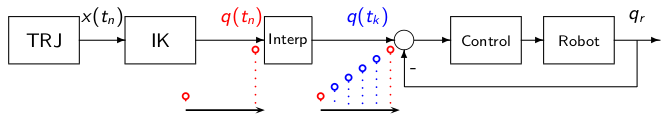
\includegraphics[width=0.65\textwidth]{worktraj}
    \end{center}
\end{figure}

For the computation of the workspace trajectories, it is possible to adopt one of the techniques used for the joint space or to define analytically the geometric path as a function of time $p=p(t)$ or, better, in a parametric form $p=p(s)$ being $s=s(t)$ a proper parameterization defining the motion law.
\subsection{Curvature of a geometric path}
Consider a path $\Gamma$ in the workspace $\mathbb{R}^3$, expressed in parametric form 
\[
    p=p(r) = \begin{bmatrix}
        x(r) \\ y(r) \\ z(r)
    \end{bmatrix}, \qquad r\in [r_a,~r_b]
\]
Assume that the curve is regular, i.e.
\[
    \dot{p} = \displaystyle\frac{d~p}{dr} \neq 0, \qquad \forall r \in [r_a,~r_b]
\]
Given a point $p_a$ of $\Gamma$, and a motion direction on the path, the \emph{arc legth} of a generic point $p(r)$ is defined as 
\[
    s = \displaystyle\int_{p_a}^{p(r)}\|\dot{p}(\rho)\|d\rho
\]
By definition, the arc length represents the legth of the arc of $\Gamma$ defined by the two points $p$ and $p_a$. The value $s=0$ is assigned to point $p_a$. 

A bijective relationship exists between the arch length $s$ and the points of the path $\Gamma$, and it is therefore possible to use the arc legnth for a parametric expression of $\Gamma$.
\[
    p=p(s)
\]
It is possible to assign to each point $p$ of $\Gamma$ a reference frame (Frenet frame) defined by the following unit vectors: 
\[
    \left\{\begin{array}{llll}
            t & = & \displaystyle\frac{\dot{p}}{\|\dot{p}\|} & \text{tangent unit vector}\\
            b & = & \displaystyle\frac{\dot{p}\times \ddot{p}}{\|\dot{p} \times \ddot{p}\|} & \text{binormal unit vector}\\
            n & = & b\times t & \text{normal unit vector}
    \end{array}\right.
\]
\subsection{Position trajectories}
\subsubsection{Segment of a line}
The linear geometric path between points $p_i$ and $p_f$ has a parametric representation expressed by 
\[
    p(s) = p_i + \displaystyle\frac{s}{\|p_f-p_i\|}(p_f-p_i) \qquad s \in [0,~\|p_f-p_i\|]
\]
Moreover, by deriving $p$ with respect to $s$, one obtains 
\[
    \displaystyle\frac{d~p}{ds}= \displaystyle\frac{p_f-p_i}{\|p_f-p_i\|}, \qquad \displaystyle\frac{d^2~p}{ds^2}=0
\]
It is possible to plan a trajectory through a sequence of points with the same modalities seen in the joint space. If it is required to pass exactly through the intermediate points, then it is possible to compute the parameter $s$ using one of the motion laws defined in the joint space. In case it is not required for the manipulator to pass through the intermediate points, the geometric path can be defined for example by linear segments with polynomial blends.
\subsubsection{Arc of a circle}
A parametric representation of an arc of a circle is 
\[
    p=p(r) = \begin{bmatrix}
        x \\ y \\ z
    \end{bmatrix} = \begin{bmatrix}
    r \cos{\theta} \\r \sin{\theta} \\ 0
    \end{bmatrix}
\]
where the parameter is the angle $\theta= \theta(t)\in[\theta_{min},\theta_{max}]$. Notice that if the path must be arbitrarily positioned/oriented in the 3D space, it is sufficient to multiply the homogenous vector $p$ by a proper transformation matrix $T$
\subsection{Rotational trajectories}





\section{Analysis of Trajectories}
When designing the control system of a robot, or more in general of an automatic machine, it is necessary to pay particular attention to the choice and design of the desired trajectory for the actuation system. As a matter of fact, a wrong choice has strong impacts on the performance, stress, and possible damages of the whole machine. In the following, two aspects will be analyzed:\begin{itemize}
    \item vibrations induced on the mechanical structure (frequency analysis of trajectories)
    \item working conditions of the actuators (trajectories and torque-speed characteristics)
\end{itemize}

\subsection{Frequency analysis of trajectories}
Vibrations are undesired phenomena often present in automatic machines. They are basically due to the presence of structural elasticity in the mechanical system, and may be generated during the normal working cycle of the machine due to several reasons. 

In particular, vibrations may be produced if trajectories with a discontinuous acceleration profile are imposed to the actuation system. 
\begin{itemize}
    \item Acceleration discontinuities $\rightarrow$ sudden variation of the inertial forces applied to the system. 
        \item Relevant discontinuities of such forces, applied to an elastic system (i.e. any mechanical device), generate vibrational effects 
            \item Since every mechanism is characterized by some elasticity, this type of phenomenon must always be considered in the design of a trajectory, that therefore should have a smooth acceleration profile or, more in general, a limited bandwidth.
\end{itemize}

Let us consider a feedback control system:
\begin{figure}[H]
    \begin{center}
        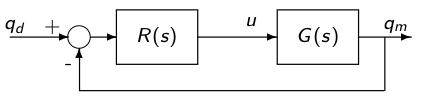
\includegraphics[width=0.65\textwidth]{compsens}
    \end{center}
\end{figure}
It is well known that, in order to have negligible tracking error, it is necessary that the spectrum of the signal $q_d(t)$ is within the bandwidth of the complementary sensitivity function 
\[
    F(s)=\displaystyle\frac{Q_d(s)}{Q_m(s)}=\displaystyle\frac{L(s)}{1+L(s)}=\displaystyle\frac{R(s)G(s)}{1+R(s)G(s)}
\]

With the current performances of electric drives, if the controller is designed in a satisfactory manner, we can expect the motor to follow with (almost) zero error the desired set-point. In case of infinitely rigid systems the load will track the desired motion exactly. If there are elastic effects in the transmission system, or more in general in case the load is not a rigid body, a different behaviour is obtained. 
Dynamic model ($\tilde{q}=q_l-q_m\approx q_l-q_d$):
\begin{gather*}
    m\ddot{q}_l+b\dot{q}_l+kq_l = b\dot{q}_m+kq_m\\
    m\ddot{\tilde{q}}_l+b\dot{\tilde{q}}_l+k\tilde{q}_l = -m\ddot{q}_m\\
    \ddot{\tilde{q}}+2\delta_z\omega_z\dot{\tilde{q}}+\omega_z^2\tilde{q} = -\ddot{q}_m
\end{gather*}
In order to avoid oscillations, the maximum frequency of the trajectory must be smaller than the resonance frequency of the system. 

In order to compare different trajectories, and to understand the effects on a given mechanical system, it is good practice to analyze their spectrum (harmonic content), in particular that of the acceleration. For this type of analysis, a \emph{normalized} expression of the trajectory is considered, that is with a time duration $T=1$ and a unitary displacement $h=1$. Moreover, the spectra $V(\Omega)$ are referred to the variable $\Omega$ defined as 
\[
    \Omega = \displaystyle\frac{\omega}{\omega_0}, \qquad \omega_0=\displaystyle\frac{2\pi}{T}
\]
Rescaling of trajectories also nicely applies to the frequency domain. 



\[
    \begin{bmatrix}
        1 & 2 & 3 \\
        4 & 5 & 5 \\
        7 & 8 & 9
    \end{bmatrix}
\]




\end{document}
